\chapter{FTP Details}

In this part, upon the two-ubuntu LAN that we built previously, we use
FTP (File transfer protocol) to transfer a 7353 bytes file from host
to server. And using Wireshark, I will give a detailed analysis on how
the ftp files break into packets and into bits.

\begin{figure}[ht!]
\centering
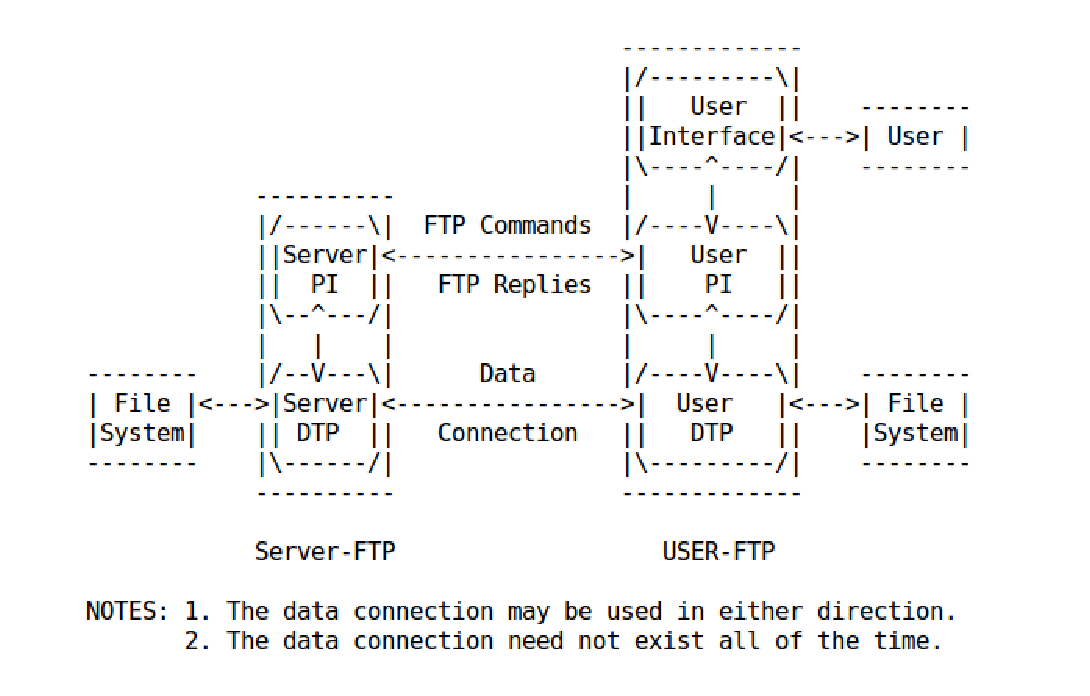
\includegraphics[scale=0.75]{eps/ftp-model.eps}
\caption{The FTP model}
\label{ftp-model}
\end{figure}

As can be seen in Figure~\ref{ftp-model}, the data connection is established
between the server DTP (data transfer process) and the user DTP, as
for ftp commands and replies, they are transfered between server PI
(protocol interpreter) and user PI.

\begin{figure}[ht!]
\centering
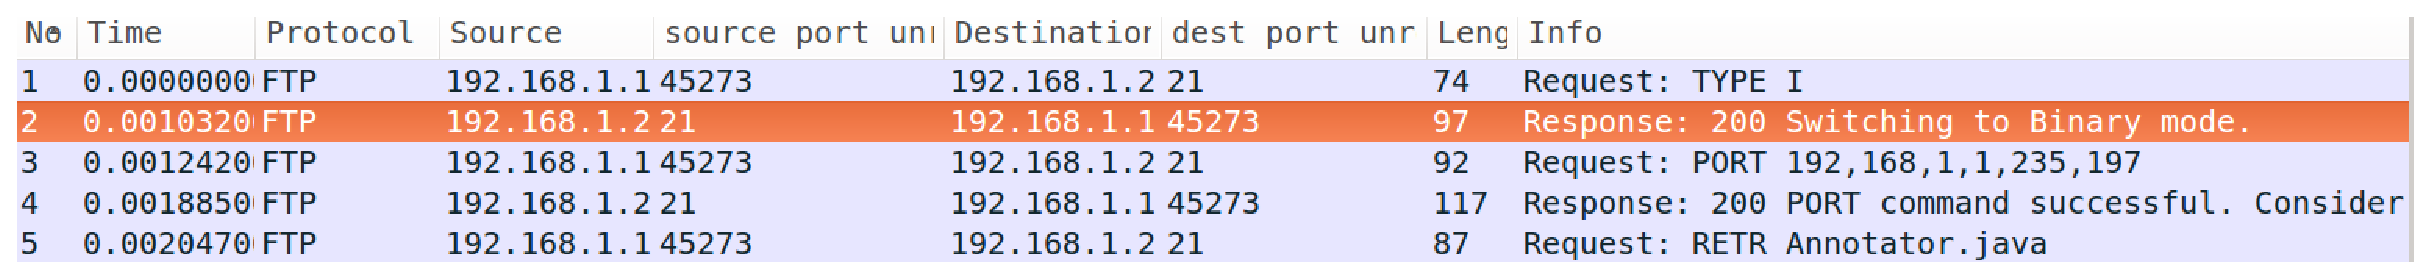
\includegraphics[scale=0.35]{eps/ftp1.eps}
\caption{FTP data connection establishment}
\label{ftp1}
\end{figure}

Figure~\ref{ftp1} shows a typical ftp data connection establishment. 
\begin{enumerate}
\item host request server for connection.
\item server responses code 200, meaning that connection permmitted.
\item and port 179,6 (45830) is to be used
\item use PASV, a mode where the client initiates the data connection.
\item ready to return the aimed file Annotator.java.
\end{enumerate}

\begin{figure}[ht!]
\centering
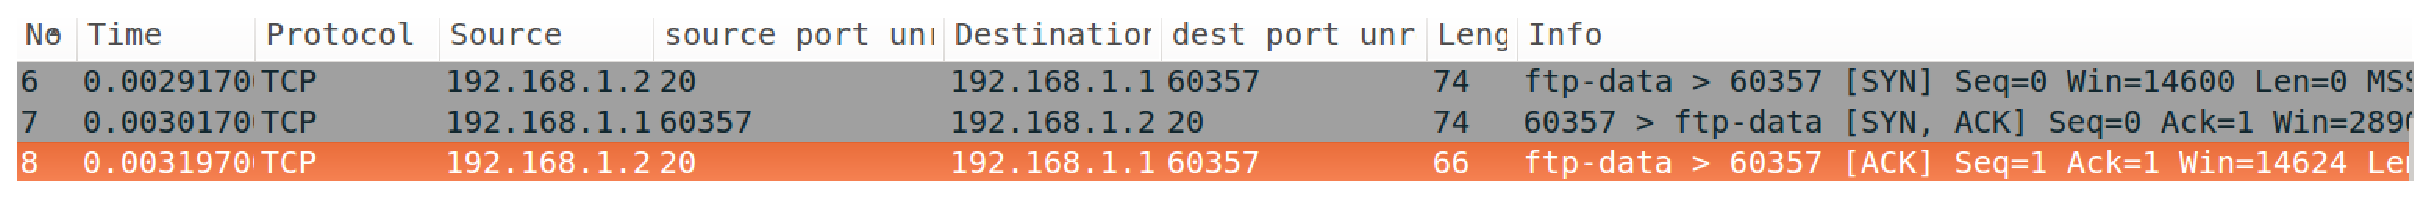
\includegraphics[scale=0.35]{eps/ftp2.eps}
\caption{A 3-way TCP handshake}
\label{ftp2}
\end{figure}

Figure~\ref{ftp2} is a typical 3-way-hand-shaking TCP, to synthesize and
establish a reliable connection.

\begin{figure}[ht!]
\centering
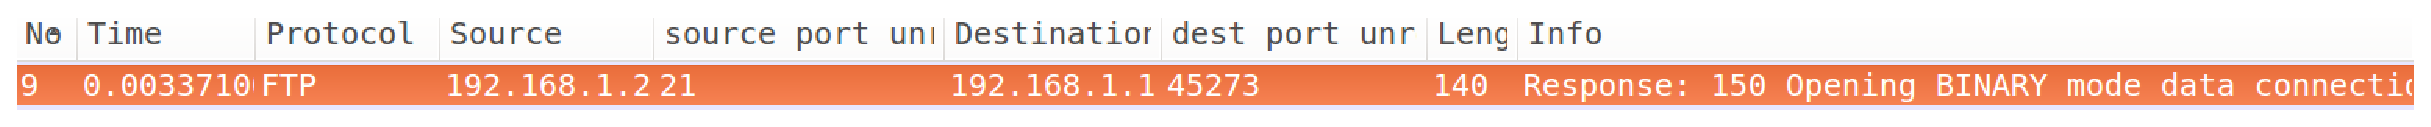
\includegraphics[scale=0.35]{eps/ftp3.eps}
\caption{File status okay, open data connection}
\label{ftp3}
\end{figure}

Figure~\ref{ftp3} shows that, code 150 means "File status okay; about to open
data connection."

\begin{figure}[ht!]
\centering
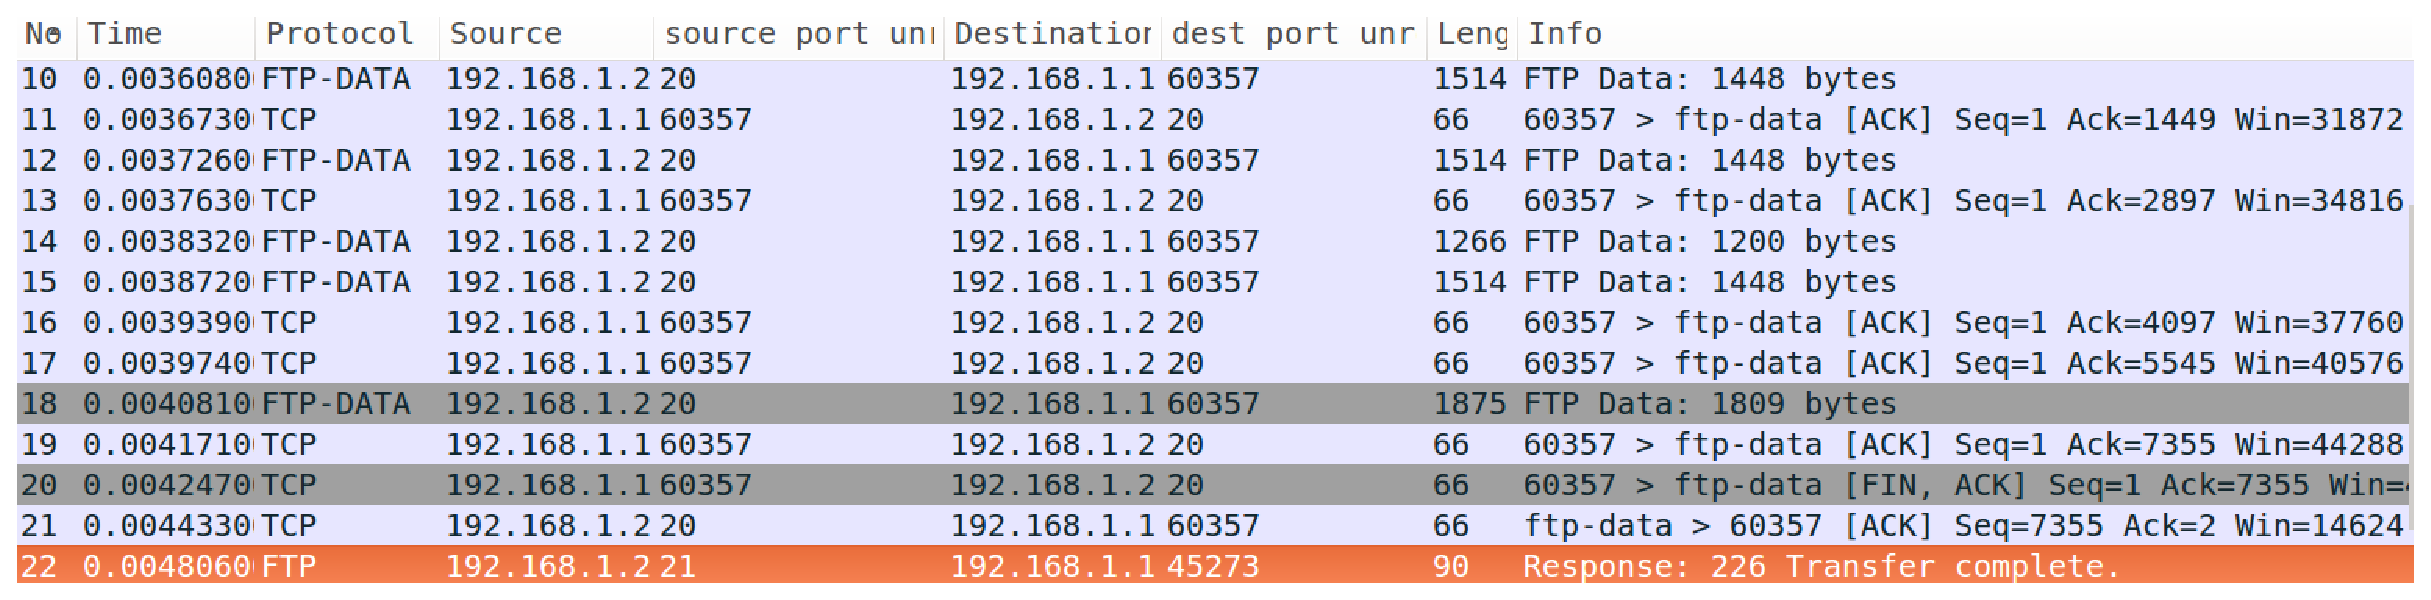
\includegraphics[scale=0.35]{eps/ftp4.eps}
\caption{File transfer}
\label{ftp4}
\end{figure}

In Figure~\ref{ftp4} 
we come to the file transfers, we can see that the files are
transferred in several parts, and after each part of data transferred
into user, user would send an ACK (acknowledgement) back to server,
meaning that the user received the data successfully. At the end, code
226 means "Closing data connection. Requested file action successful
(for example, file transfer or file abort)."

\begin{figure}[ht!]
\centering
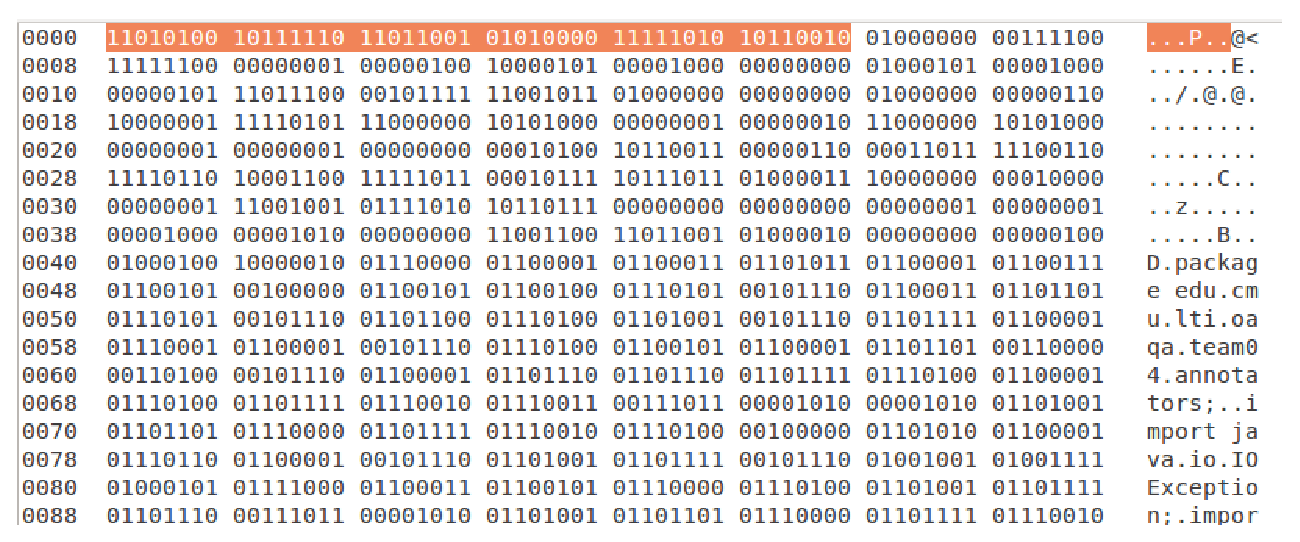
\includegraphics[scale=0.65]{eps/ftp5.eps}
\caption{An FTP data packet}
\label{ftp5}
\end{figure}

Figure~\ref{ftp5} shows one of the ftp-data packet, where bits of the packet
can be seen.

First, how can we know if the packet is the ftp-data packet? We can
check the source port (20 as ftp data) and destination port, and in
the meantime check if there are bits after 66 bytes. (We will see the
code inplementation of this soon)

Thus, similarly, for every ftp-data packet, we can grab those bits of
data from the 66 bytes of the packet to the end.

Now let's look into the bits of one of the ftp-data packet of the file
(Annotator.java).

\begin{figure}[ht!]
\centering
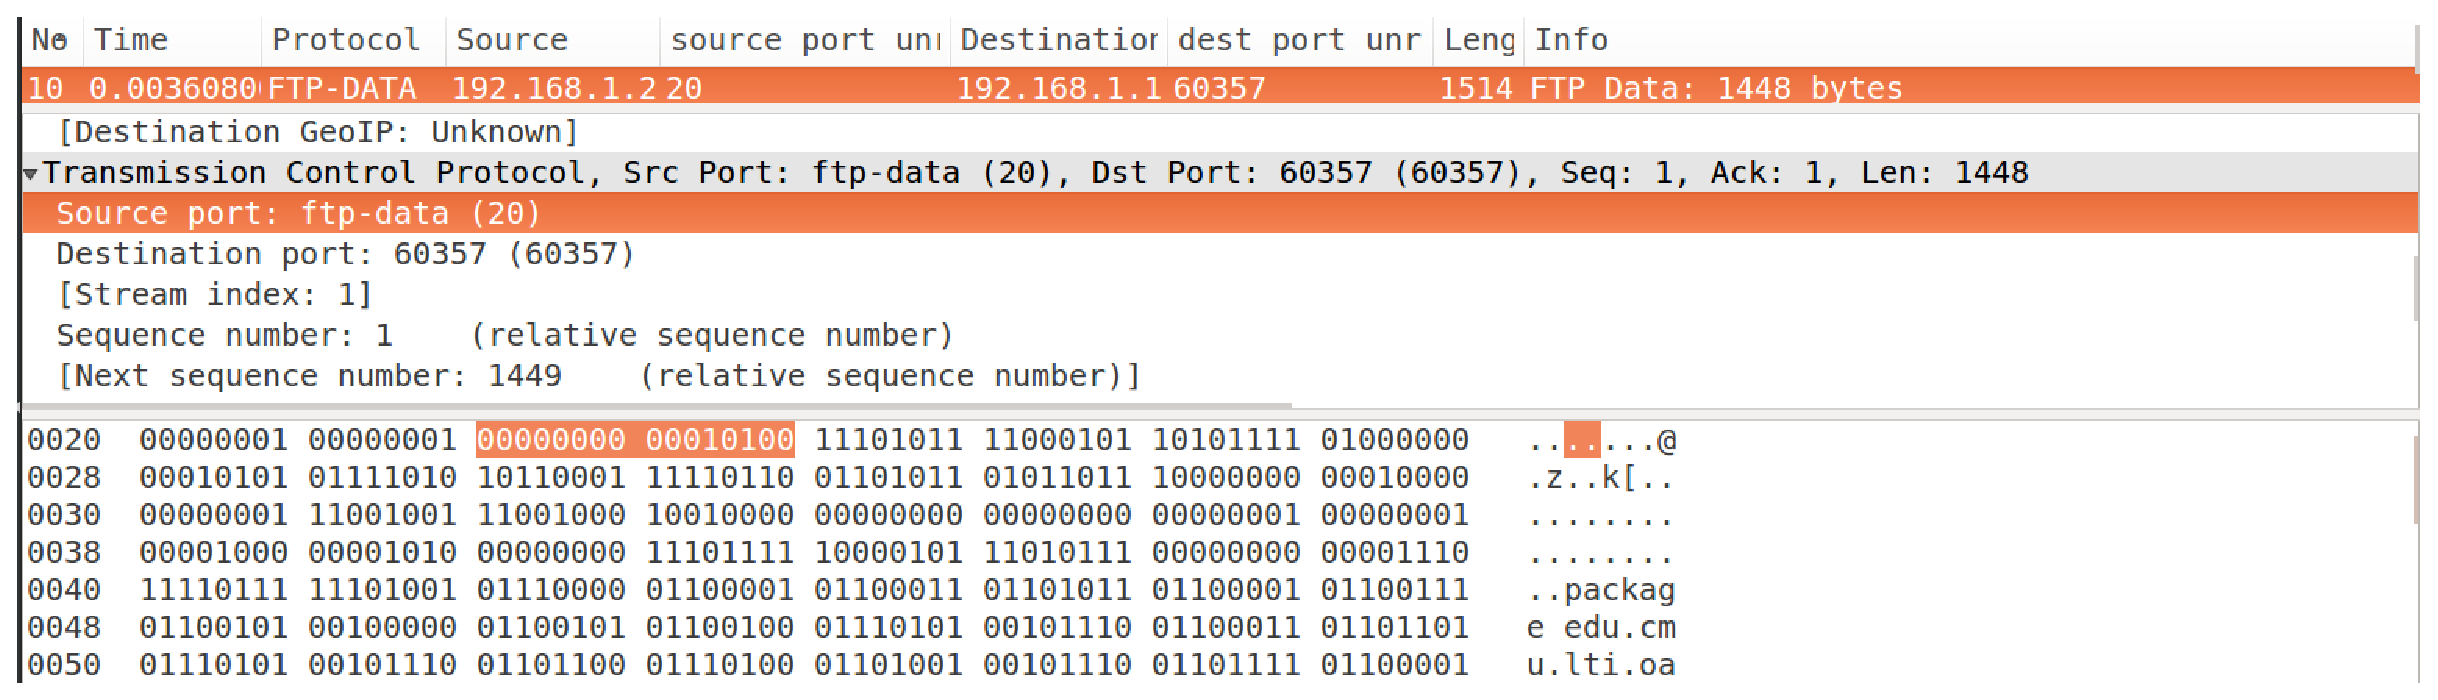
\includegraphics[scale=0.35]{eps/ftp6.eps}
\caption{Details}
\label{ftp6}
\end{figure}

Figure~\ref{ftp6}, figure~\ref{ftp7}, figure~\ref{ftp8}, and 
figure~\ref{ftp9} 
show the details for a packet. 

\newpage
For each packet:

\begin{figure}[ht!]
\centering
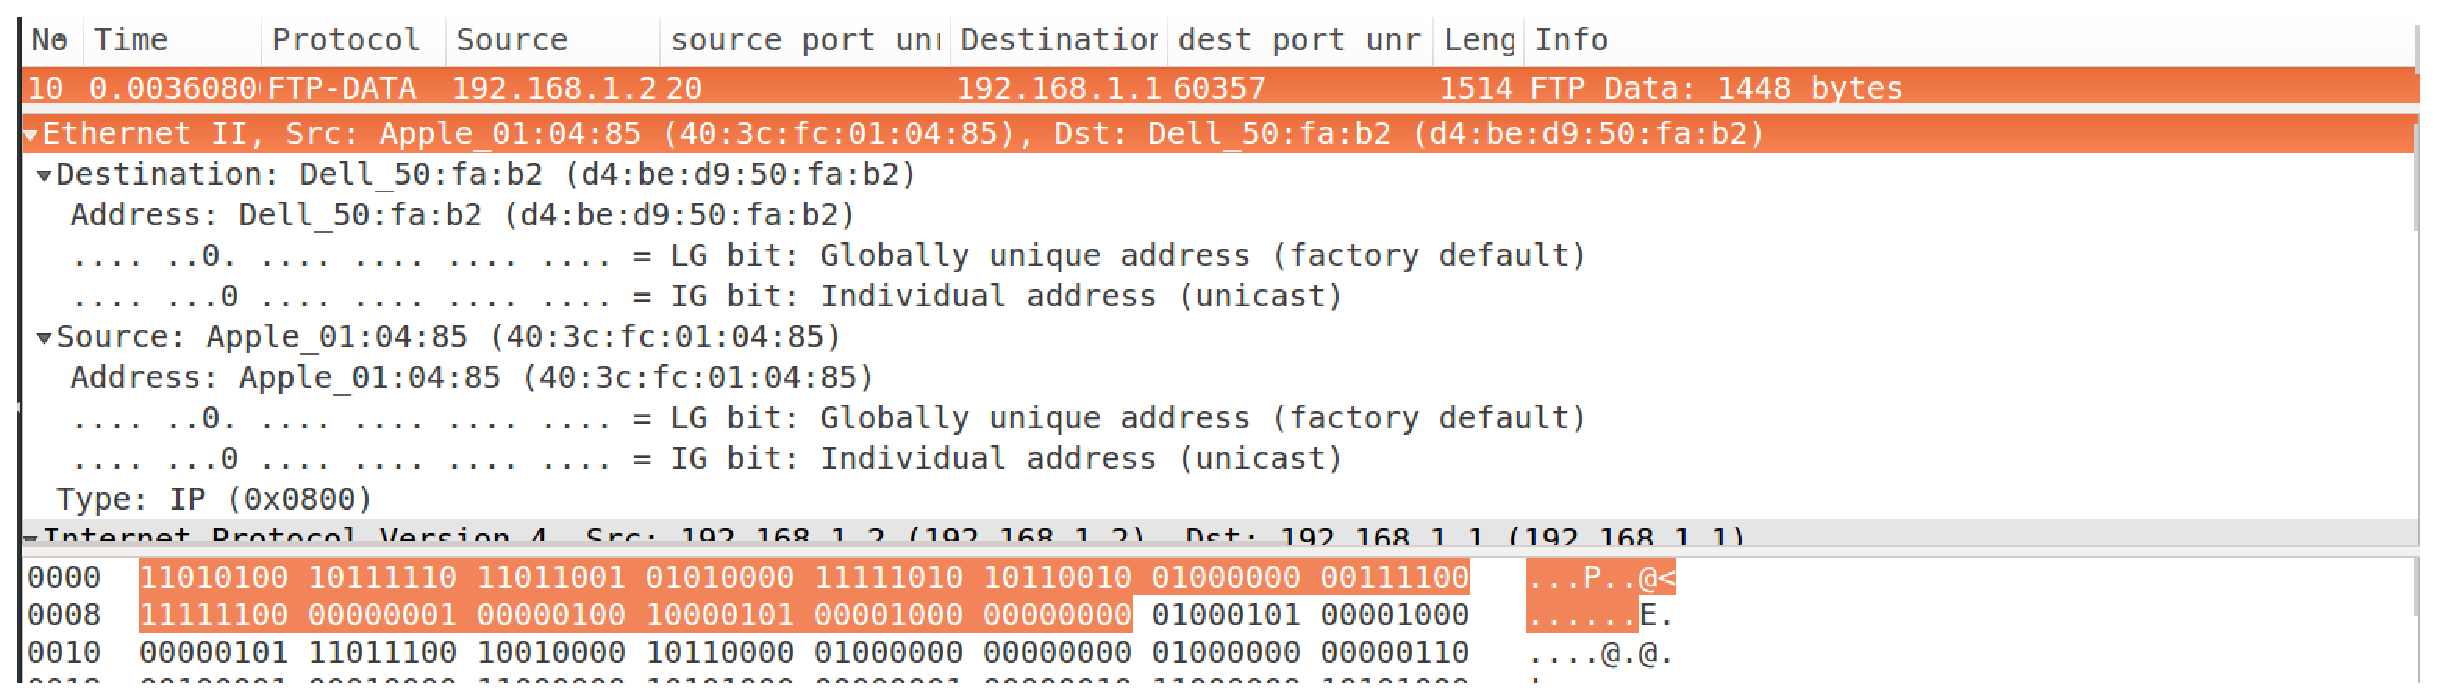
\includegraphics[scale=0.35]{eps/ftp7.eps}
\caption{Bit level details}
\label{ftp7}
\end{figure}

\begin{enumerate}
\item {\bf bytes 0-5} first 6 bytes are user mac 
address (d4:be:d9:50:fa:b2 here)

\begin{chunk}{get dest mac addr}
/*got to write this*/
\end{chunk}

{\bf bytes 6-11} (6) bytes are server mac 
address (40:3c:fc:01:04:85), 

{\bf bytes 12-13} (2) bytes are IP (0X0800).

\newpage
\begin{figure}[ht!]
\centering
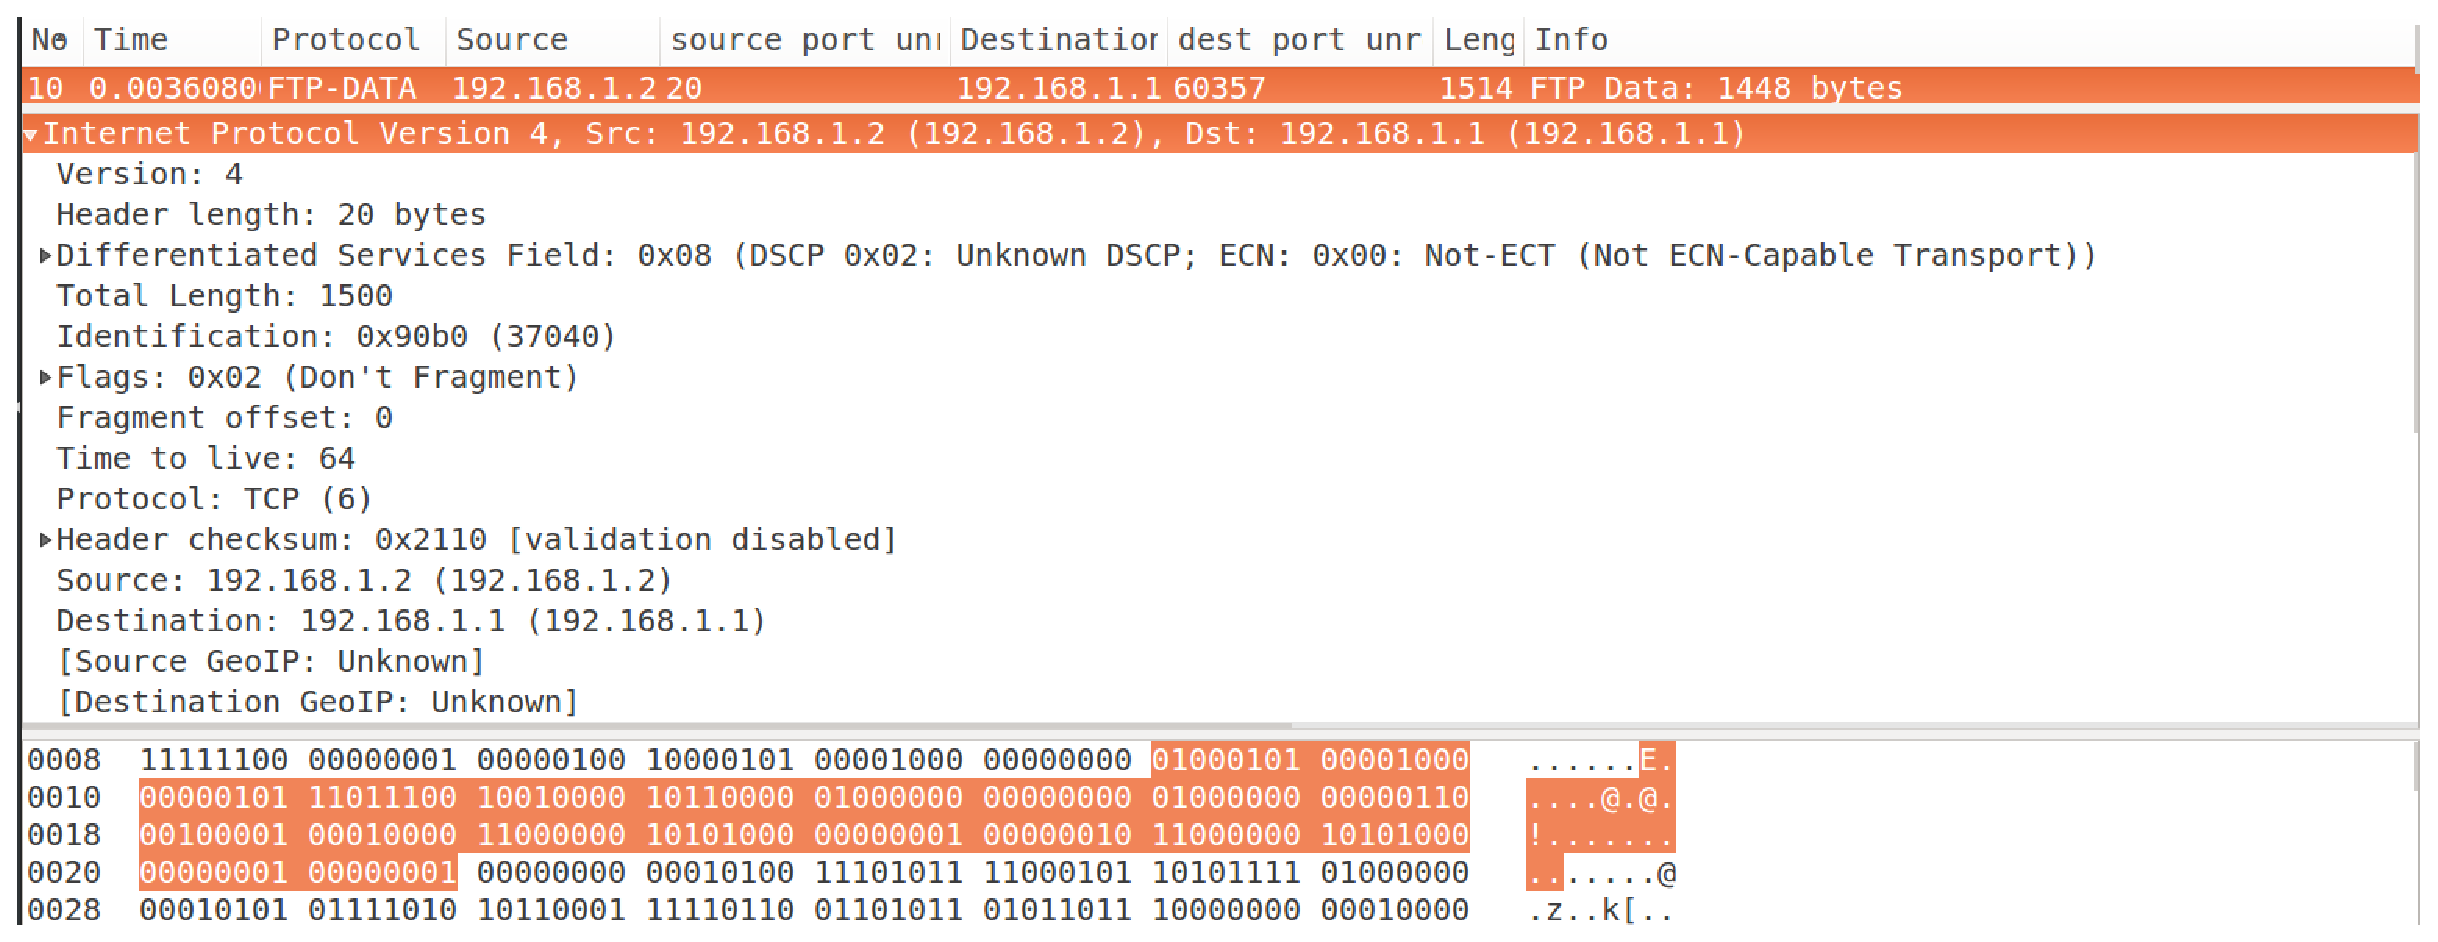
\includegraphics[scale=0.35]{eps/ftp8.eps}
\caption{More bit level details}
\label{ftp8}
\end{figure}

\item {\bf byte 14} is header length (20), 

{\bf byte 15} is the tag byte, 

{\bf bytes 16-17} (2) bytes are total length of data transferred (1500), 

{\bf bytes 18-19} (2) bytes are identification (0x2fcb $->$ 12235), 

{\bf bytes 20-21} (2) bytes are fragment offset (0), 

{\bf byte 22} is time to live (64), 

{\bf byte 23} is protocol used (6 $->$ TCP),

{\bf bytes 24-25} (2) bytes are header checksum 
(0x81f5 $->$ validation disabled),

{\bf bytes 26-29} (4) bytes are source GeoIP (unknown), 

{\bf bytes 30-33} (4) bytes are destination GeoIP (unknown).

\newpage
\begin{figure}[ht!]
\centering
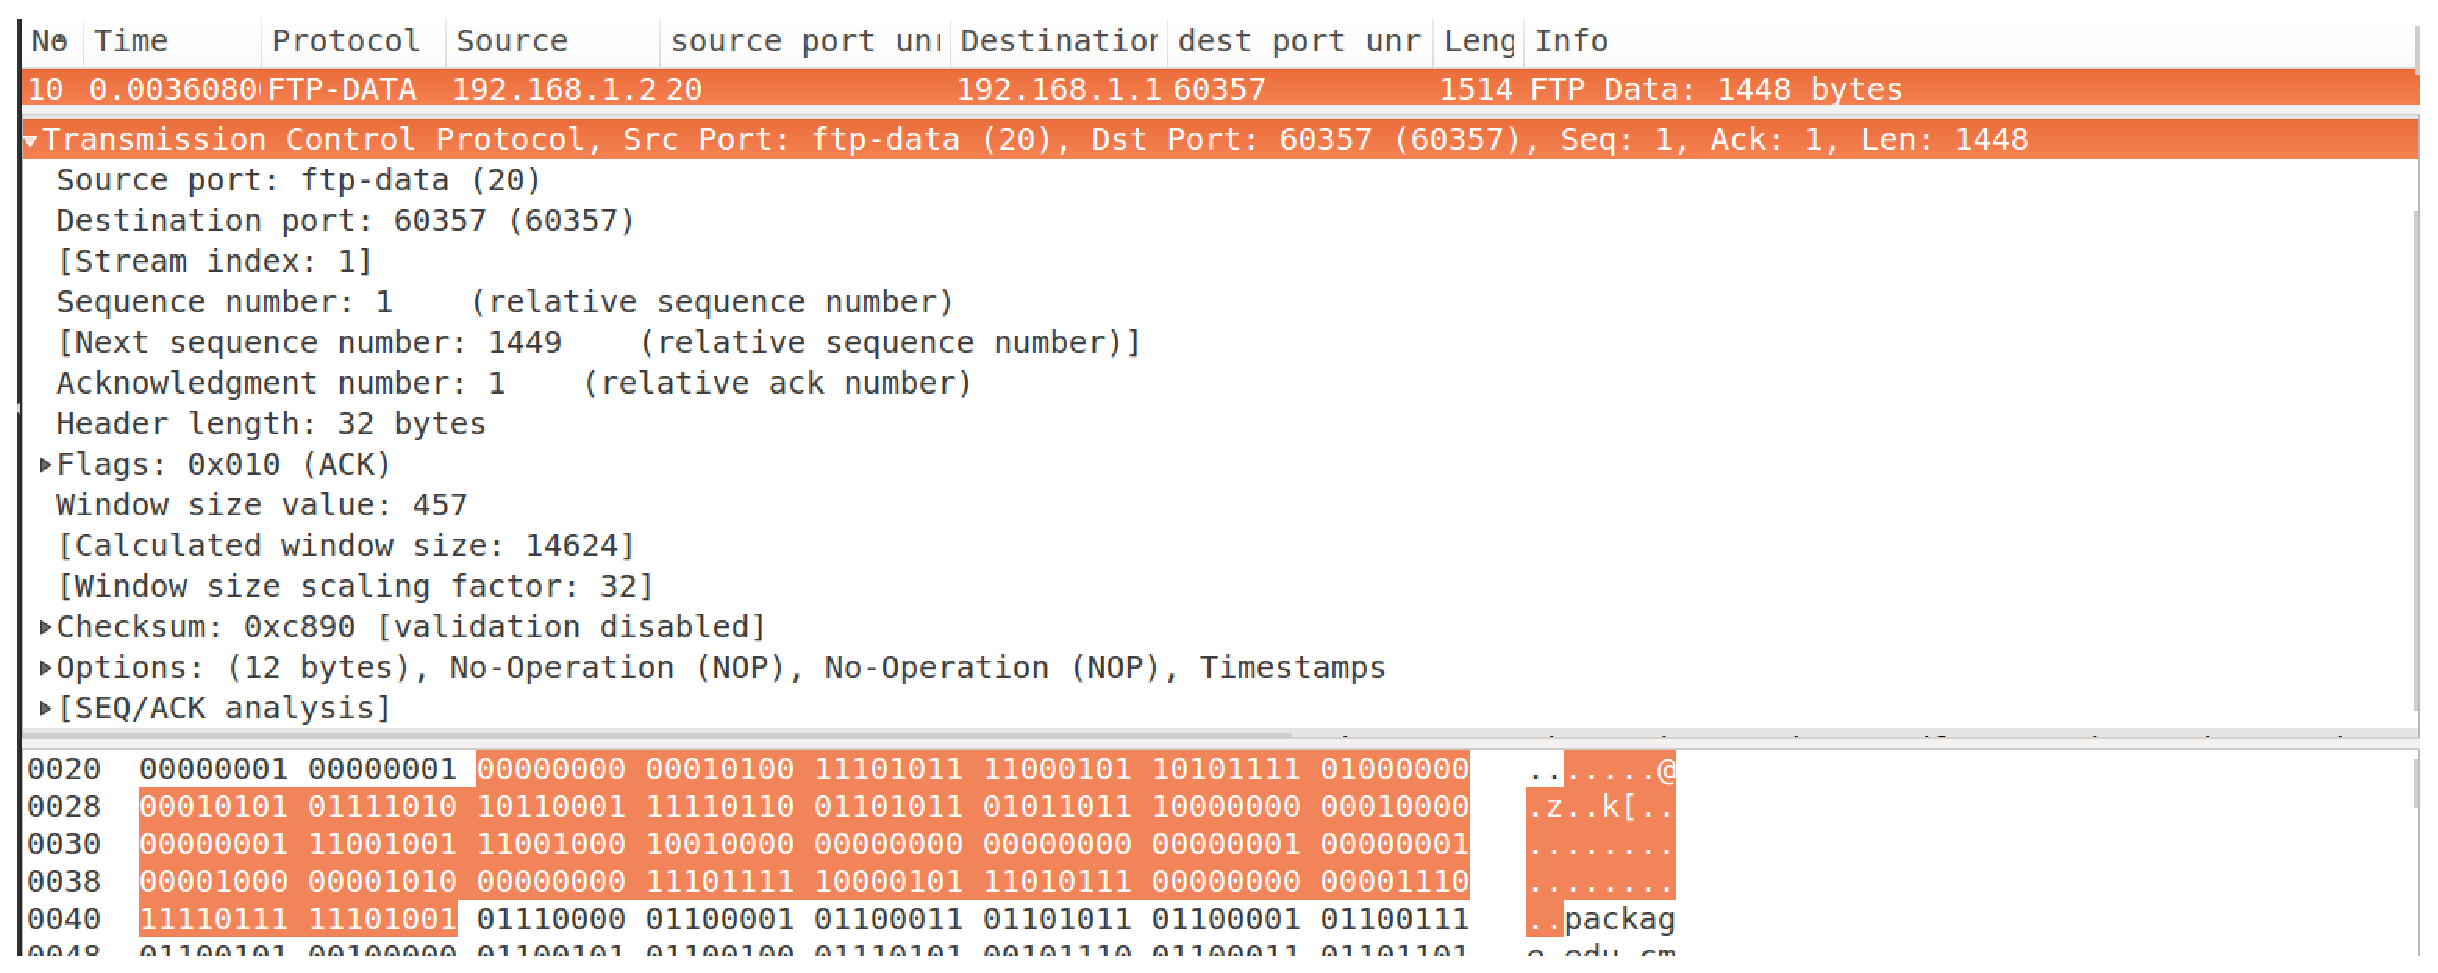
\includegraphics[scale=0.35]{eps/ftp9.eps}
\caption{More bit level details}
\label{ftp9}
\end{figure}

\item {\bf bytes 34-35} (2) bytes are source port (20 $->$ ftp-data port), 

{\bf bytes 36-37} (2) bytes are destination port (45830), 

{\bf bytes 38-41} (4) bytes are sequence number (1), 

{\bf bytes 42-45} (4) bytes are acknowledgment number (1), 

{\bf bytes 46-47} (2) bytes are flags (0x010), 

{\bf bytes 48-49} (2) bytes are window size value and scaling factor, 

{\bf bytes 50-51} (2) bytes are checksum (0x7ab7 $->$ validation
disabled), 

{\bf bytes 52-61} all belong to TCP, 

{\bf bytes 62-65} (4) bytes are timestamp echo reply (279682).

\item then we see our data (1448 bytes), 
which takes a large part of the packet.
\end{enumerate}

Thus, this analysis gives us the hint of how to abstract the bits of
the file out of the packets flow.

A packet analyzer (also known as a network analyzer, protocol analyzer
or packet sniffer—or, for particular types of networks, an Ethernet
sniffer or wireless sniffer) is a computer program or piece of
computer hardware that can intercept and log traffic that passes over
a digital network or part of a network. As data streams flow across
the network, the sniffer captures each packet and, if needed, decodes
the packet's raw data, showing the values of various fields in the
packet, and analyzes its content according to the appropriate RFC or
other specifications. \cite{39} Wireshark for example is the most
popular packet sniffer out there and is available for all
platforms. Its gui based and very easy to use.

In this chapter we are going to talk about how to code and make our own packet sniffer in C and on the linux platform. 

Note that it sniffs only incoming packets.

\begin{chunk}{includes}
#include<stdio.h> //For standard things
#include<stdlib.h>    //malloc
#include<string.h>    //memset
//can get
#include<netinet/tcp.h>   //Provides declarations for tcp header
//can get
#include<netinet/ip.h>    //Provides declarations for ip header
#include<sys/socket.h>
#include<arpa/inet.h>

\end{chunk}

\begin{chunk}{About the sockaddrin struct}
struct sockaddr_in{
  short sin_family;
  unsigned short sin_port;
  IN_ADDR sin_addr;
  char sin_zero[8];
};
members in struct:
sin_family
    Address family; must be AF_INET.
sin_port
    Internet Protocol (IP) port.
sin_addr
    IP address in network byte order.
sin_zero
    Padding to make structure the same size as SOCKADDR.
\end{chunk}

\begin{chunk}{globalVs}
int sock_raw;
FILE *logfile;
int tcp=0,others=0,total=0,i,j;
struct sockaddr_in source,dest;

\end{chunk}

\noindent
Function prototypes
\begin{chunk}{prototypes}
void ProcessPacket(unsigned char* , int);
void printipheader(unsigned char* , int);
void printtcppacket(unsigned char* , int);
void PrintData (unsigned char* , int);

\end{chunk}

\subsection{The ProcessPacket function}
\index{ProcessPacket}
\index{function!ProcessPacket}
\noindent
In this ProcessPacket function, we:

1. get the IP header part of the packet.
2. check the protocol and see if it's tcp in this case
3. if it's tcp, then print the packet in tcp format

\begin{chunk}{ProcessPacket}
void ProcessPacket(unsigned char* buffer, int size)
{
    //Get the IP Header part of this packet
    struct iphdr *iph = (struct iphdr*)buffer;
    ++total;
    switch (iph->protocol) //Check the Protocol and do accordingly...
    { 
        case 6:  //TCP Protocol
            ++tcp;
            printtcppacket(buffer , size);
            break;
         
        default: //Some Other Protocol like ARP etc.
            ++others;
            break;
    }
    printf("TCP : %d   Others : %d   Total : %d\r",tcp,others,total);
}

\end{chunk}

\subsection{The printipheader function}
\index{printipheader}
\index{function!printipheader}
For {\bf printipheader}, 

\begin{chunk}{printipheader}
void printipheader(unsigned char* Buffer, int Size)
{
    unsigned short iphdrlen;
         
    struct iphdr *iph = (struct iphdr *)Buffer;
    iphdrlen =iph->ihl*4;
     
    memset(&source, 0, sizeof(source));
    source.sin_addr.s_addr = iph->saddr;
     
    memset(&dest, 0, sizeof(dest));
    dest.sin_addr.s_addr = iph->daddr;
     
    fprintf(logfile,"\n");
    fprintf(logfile,"IP Header\n");
    fprintf(logfile,"   |-IP Version        : %d\n",(unsigned int)iph->version);
    fprintf(logfile,"   |-IP Header Length  : %d DWORDS or %d Bytes\n",(unsigned int)iph->ihl,((unsigned int)(iph->ihl))*4);
    fprintf(logfile,"   |-Type Of Service   : %d\n",(unsigned int)iph->tos);
    fprintf(logfile,"   |-IP Total Length   : %d  Bytes(Size of Packet)\n",ntohs(iph->tot_len));
    fprintf(logfile,"   |-Identification    : %d\n",ntohs(iph->id));
    //fprintf(logfile,"   |-Reserved ZERO Field   : %d\n",(unsigned int)iphdr->ip_reserved_zero);
    //fprintf(logfile,"   |-Dont Fragment Field   : %d\n",(unsigned int)iphdr->ip_dont_fragment);
    //fprintf(logfile,"   |-More Fragment Field   : %d\n",(unsigned int)iphdr->ip_more_fragment);
    fprintf(logfile,"   |-TTL      : %d\n",(unsigned int)iph->ttl);
    fprintf(logfile,"   |-Protocol : %d\n",(unsigned int)iph->protocol);
    fprintf(logfile,"   |-Checksum : %d\n",ntohs(iph->check));
    fprintf(logfile,"   |-Source IP        : %s\n",inet_ntoa(source.sin_addr));
    fprintf(logfile,"   |-Destination IP   : %s\n",inet_ntoa(dest.sin_addr));
}

\end{chunk}

\subsection{The printtcppacket function}
\index{printtcppacket}
\index{function!printtcppacket}
The {\bf printtcppacket} will 
\begin{chunk}{printtcppacket}
void printtcppacket(unsigned char* Buffer, int Size)
{
    unsigned short iphdrlen;
     
    struct iphdr *iph = (struct iphdr *)Buffer;
    iphdrlen = iph->ihl*4;
     
    struct tcphdr *tcph=(struct tcphdr*)(Buffer + iphdrlen);
             
    fprintf(logfile,"\n\n***********************TCP Packet*************************\n");   
         
    printipheader(Buffer,Size);
         
    fprintf(logfile,"\n");
    fprintf(logfile,"TCP Header\n");
    fprintf(logfile,"   |-Source Port      : %u\n",ntohs(tcph->source));
    fprintf(logfile,"   |-Destination Port : %u\n",ntohs(tcph->dest));
    fprintf(logfile,"   |-Sequence Number    : %u\n",ntohl(tcph->seq));
    fprintf(logfile,"   |-Acknowledge Number : %u\n",ntohl(tcph->ack_seq));
    fprintf(logfile,"   |-Header Length      : %d DWORDS or %d BYTES\n" ,(unsigned int)tcph->doff,(unsigned int)tcph->doff*4);
    //fprintf(logfile,"   |-CWR Flag : %d\n",(unsigned int)tcph->cwr);
    //fprintf(logfile,"   |-ECN Flag : %d\n",(unsigned int)tcph->ece);
    fprintf(logfile,"   |-Urgent Flag          : %d\n",(unsigned int)tcph->urg);
    fprintf(logfile,"   |-Acknowledgement Flag : %d\n",(unsigned int)tcph->ack);
    fprintf(logfile,"   |-Push Flag            : %d\n",(unsigned int)tcph->psh);
    fprintf(logfile,"   |-Reset Flag           : %d\n",(unsigned int)tcph->rst);
    fprintf(logfile,"   |-Synchronise Flag     : %d\n",(unsigned int)tcph->syn);
    fprintf(logfile,"   |-Finish Flag          : %d\n",(unsigned int)tcph->fin);
    fprintf(logfile,"   |-Window         : %d\n",ntohs(tcph->window));
    fprintf(logfile,"   |-Checksum       : %d\n",ntohs(tcph->check));
    fprintf(logfile,"   |-Urgent Pointer : %d\n",tcph->urg_ptr);
    fprintf(logfile,"\n");
    fprintf(logfile,"                        DATA Dump                         ");
    fprintf(logfile,"\n");
         
    fprintf(logfile,"IP Header\n");
    PrintData(Buffer,iphdrlen);
         
    fprintf(logfile,"TCP Header\n");
    PrintData(Buffer+iphdrlen,tcph->doff*4);
         
    fprintf(logfile,"Data Payload\n"); 
    PrintData(Buffer + iphdrlen + tcph->doff*4 , (Size - tcph->doff*4-iph->ihl*4) );
                         
    fprintf(logfile,"\n###########################################################");
}

\end{chunk}

\subsection{The PrintData function}
\label{PrintData}
\index{PrintData}
\index{function!PrintData}
The {\bf PrintData} will 

\begin{chunk}{PrintData}
void PrintData (unsigned char* data , int Size)
{
     
    for(i=0 ; i < Size ; i++)
    {
        if( i!=0 && i%16==0)   //if one line of hex printing is complete...
        {
            fprintf(logfile,"         ");
            for(j=i-16 ; j<i ; j++)
            {
                if(data[j]>=32 && data[j]<=128)
                    fprintf(logfile,"%c",(unsigned char)data[j]); //if its a number or alphabet
                 
                else fprintf(logfile,"."); //otherwise print a dot
            }
            fprintf(logfile,"\n");
        }
         
        if(i%16==0) fprintf(logfile,"   ");
            fprintf(logfile," %02X",(unsigned int)data[i]);
                 
        if( i==Size-1)  //print the last spaces
        {
            for(j=0;j<15-i%16;j++) fprintf(logfile,"   "); //extra spaces
             
            fprintf(logfile,"         ");
             
            for(j=i-i%16 ; j<=i ; j++)
            {
                if(data[j]>=32 && data[j]<=128) fprintf(logfile,"%c",(unsigned char)data[j]);
                else fprintf(logfile,".");
            }
            fprintf(logfile,"\n");
        }
    }
}

\end{chunk}

\subsection{ear.c}
\index{main}
\index{function!main}
\noindent
The {\bf main} function 

In the main() function we:

1. Create a raw socket, using socket() function.
2. Put it in a recvfrom loop and receive data on it, and process the recieved data.
3. close the socket after at the end.


\begin{chunk}{ear.c}

\getchunk{includes}
\getchunk{globalVs}
\getchunk{prototypes}
\getchunk{ProcessPacket}
\getchunk{printipheader}
\getchunk{printtcppacket}
\getchunk{PrintData}

int main()
{
    int saddr_size , data_size;
    struct sockaddr saddr;
    struct in_addr in;
     
    unsigned char *buffer = (unsigned char *)malloc(65536); //Its Big!
     
    logfile=fopen("log.txt","w");
    if(logfile==NULL) printf("Unable to create file.");
    printf("Starting...\n");
    //Create a raw socket that shall sniff
    sock_raw = socket(AF_INET , SOCK_RAW , IPPROTO_TCP);
    if(sock_raw < 0)
    {
        printf("Socket Error\n");
        return 1;
    }
    while(1)
    {
        saddr_size = sizeof saddr;
        //Receive a packet
        data_size = recvfrom(sock_raw , buffer , 65536 , 0 , &saddr , &saddr_size);
        if(data_size <0 )
        {
            printf("Recvfrom error , failed to get packets\n");
            return 1;
        }
        //Now process the packet
        ProcessPacket(buffer , data_size);
    }
    close(sock_raw);
    printf("Finished");
    return 0;
}

\end{chunk}

\begin{chunk}{sample output:}

***********************TCP Packet*************************

IP Header
   |-IP Version        : 4
   |-IP Header Length  : 5 DWORDS or 20 Bytes
   |-Type Of Service   : 8
   |-IP Total Length   : 1500  Bytes(Size of Packet)
   |-Identification    : 1652
   |-TTL      : 64
   |-Protocol : 6
   |-Checksum : 43852
   |-Source IP        : 192.168.1.2
   |-Destination IP   : 192.168.1.1

TCP Header
   |-Source Port      : 20
   |-Destination Port : 59325
   |-Sequence Number    : 110330488
   |-Acknowledge Number : 1095205422
   |-Header Length      : 8 DWORDS or 32 BYTES
   |-Urgent Flag          : 0
   |-Acknowledgement Flag : 1
   |-Push Flag            : 0
   |-Reset Flag           : 0
   |-Synchronise Flag     : 0
   |-Finish Flag          : 0
   |-Window         : 457
   |-Checksum       : 59494
   |-Urgent Pointer : 0

                        DATA Dump                         
IP Header
    45 08 05 DC 06 74 40 00 40 06 AB 4C C0 A8 01 02         E....t@.@..L....
    C0 A8 01 01                                             ....
TCP Header
    00 14 E7 BD 06 93 82 78 41 47 82 2E 80 10 01 C9         .......xAG..€...
    E8 66 00 00 01 01 08 0A 01 02 84 05 00 10 F6 76         .f.............v
Data Payload
    69 6D 70 6F 72 74 20 6A 61 76 61 2E 69 6F 2E 49         import java.io.I
    4F 45 78 63 65 70 74 69 6F 6E 3B 0A 69 6D 70 6F         OException;.impo
    72 74 20 6A 61 76 61 2E 75 74 69 6C 2E 41 72 72         rt java.util.Arr
    61 79 4C 69 73 74 3B 0A 69 6D 70 6F 72 74 20 6A         ayList;.import j
    61 76 61 2E 75 74 69 6C 2E 43 6F 6C 6C 65 63 74         ava.util.Collect
    69 6F 6E 3B 0A 69 6D 70 6F 72 74 20 6A 61 76 61         ion;.import java
    2E 75 74 69 6C 2E 4C 69 73 74 3B 0A 69 6D 70 6F         .util.List;.impo
    72 74 20 6F 72 67 2E 61 70 61 63 68 65 2E 63 6F         rt org.apache.co
    6D 6D 6F 6E 73 2E 63 6F 6E 66 69 67 75 72 61 74         mmons.configurat
    69 6F 6E 2E 43 6F 6E 66 69 67 75 72 61 74 69 6F         ion.Configuratio
    6E 45 78 63 65 70 74 69 6F 6E 3B 0A 69 6D 70 6F         nException;.impo
    72 74 20 6F 72 67 2E 61 70 61 63 68 65 2E 75 69         rt org.apache.ui
    6D 61 2E 55 69 6D 61 43 6F 6E 74 65 78 74 3B 0A         ma.UimaContext;.
    69 6D 70 6F 72 74 20 6F 72 67 2E 61 70 61 63 68         import org.apach
    65 2E 75 69 6D 61 2E 61 6E 61 6C 79 73 69 73 5F         e.uima.analysis_
    63 6F 6D 70 6F 6E 65 6E 74 2E 4A 43 61 73 41 6E         component.JCasAn
    6E 6F 74 61 74 6F 72 5F 49 6D 70 6C 42 61 73 65         notator_ImplBase
    3B 0A 69 6D 70 6F 72 74 20 6F 72 67 2E 61 70 61         ;.import org.apa
    63 68 65 2E 75 69 6D 61 2E 61 6E 61 6C 79 73 69         che.uima.analysi
    73 5F 65 6E 67 69 6E 65 2E 41 6E 61 6C 79 73 69         s_engine.Analysi
    73 45 6E 67 69 6E 65 50 72 6F 63 65 73 73 45 78         sEngineProcessEx
    63 65 70 74 69 6F 6E 3B 0A 69 6D 70 6F 72 74 20         ception;.import 
    6F 72 67 2E 61 70 61 63 68 65 2E 75 69 6D 61 2E         org.apache.uima.
    63 61 73 2E 46 53 49 74 65 72 61 74 6F 72 3B 0A         cas.FSIterator;.
    69 6D 70 6F 72 74 20 6F 72 67 2E 61 70 61 63 68         import org.apach
    65 2E 75 69 6D 61 2E 6A 63 61 73 2E 4A 43 61 73         e.uima.jcas.JCas
    3B 0A 69 6D 70 6F 72 74 20 6F 72 67 2E 61 70 61         ;.import org.apa
    63 68 65 2E 75 69 6D 61 2E 6A 63 61 73 2E 63 61         che.uima.jcas.ca
    73 2E 46 53 4C 69 73 74 3B 0A 69 6D 70 6F 72 74         s.FSList;.import
    20 6F 72 67 2E 61 70 61 63 68 65 2E 75 69 6D 61          org.apache.uima
    2E 6A 63 61 73 2E 63 61 73 2E 53 74 72 69 6E 67         .jcas.cas.String
    4C 69 73 74 3B 0A 69 6D 70 6F 72 74 20 6F 72 67         List;.import org
    2E 61 70 61 63 68 65 2E 75 69 6D 61 2E 72 65 73         .apache.uima.res
    6F 75 72 63 65 2E 52 65 73 6F 75 72 63 65 49 6E         ource.ResourceIn
    69 74 69 61 6C 69 7A 61 74 69 6F 6E 45 78 63 65         itializationExce
    70 74 69 6F 6E 3B 0A 69 6D 70 6F 72 74 20 75 74         ption;.import ut
    69 6C 2E 2A 3B 0A 69 6D 70 6F 72 74 20 65 64 75         il.*;.import edu
    2E 63 6D 75 2E 6C 74 69 2E 6F 61 71 61 2E 62 69         .cmu.lti.oaqa.bi
    6F 2E 62 69 6F 61 73 71 2E 73 65 72 76 69 63 65         o.bioasq.service
    73 2E 47 6F 50 75 62 4D 65 64 53 65 72 76 69 63         s.GoPubMedServic
    65 3B 0A 69 6D 70 6F 72 74 20 65 64 75 2E 63 6D         e;.import edu.cm
    75 2E 6C 74 69 2E 6F 61 71 61 2E 62 69 6F 2E 62         u.lti.oaqa.bio.b
    69 6F 61 73 71 2E 73 65 72 76 69 63 65 73 2E 4C         ioasq.services.L
    69 6E 6B 65 64 4C 69 66 65 44 61 74 61 53 65 72         inkedLifeDataSer
    76 69 63 65 52 65 73 70 6F 6E 73 65 3B 0A 69 6D         viceResponse;.im
    70 6F 72 74 20 65 64 75 2E 63 6D 75 2E 6C 74 69         port edu.cmu.lti
    2E 6F 61 71 61 2E 62 69 6F 2E 62 69 6F 61 73 71         .oaqa.bio.bioasq
    2E 73 65 72 76 69 63 65 73 2E 4F 6E 74 6F 6C 6F         .services.Ontolo
    67 79 53 65 72 76 69 63 65 52 65 73 70 6F 6E 73         gyServiceRespons
    65 3B 0A 69 6D 70 6F 72 74 20 65 64 75 2E 63 6D         e;.import edu.cm
    75 2E 6C 74 69 2E 6F 61 71 61 2E 62 69 6F 2E 62         u.lti.oaqa.bio.b
    69 6F 61 73 71 2E 73 65 72 76 69 63 65 73 2E 50         ioasq.services.P
    75 62 4D 65 64 53 65 61 72 63 68 53 65 72 76 69         ubMedSearchServi
    63 65 52 65 73 70 6F 6E 73 65 3B 0A 69 6D 70 6F         ceResponse;.impo
    72 74 20 65 64 75 2E 63 6D 75 2E 6C 74 69 2E 6F         rt edu.cmu.lti.o
    61 71 61 2E 62 69 6F 2E 62 69 6F 61 73 71 2E 73         aqa.bio.bioasq.s
    65 72 76 69 63 65 73 2E 50 75 62 4D 65 64 53 65         ervices.PubMedSe
    61 72 63 68 53 65 72 76 69 63 65 52 65 73 70 6F         archServiceRespo
    6E 73 65 2E 44 6F 63 75 6D 65 6E 74 3B 0A 69 6D         nse.Document;.im
    70 6F 72 74 20 65 64 75 2E 63 6D 75 2E 6C 74 69         port edu.cmu.lti
    2E 6F 61 71 61 2E 74 79 70 65 2E 69 6E 70 75 74         .oaqa.type.input
    2E 51 75 65 73 74 69 6F 6E 3B 0A 69 6D 70 6F 72         .Question;.impor
    74 20 65 64 75 2E 63 6D 75 2E 6C 74 69 2E 6F 61         t edu.cmu.lti.oa
    71 61 2E 74 79 70 65 2E 6B 62 2E 43 6F 6E 63 65         qa.type.kb.Conce
    70 74 3B 0A 69 6D 70 6F 72 74 20 65 64 75 2E 63         pt;.import edu.c
    6D 75 2E 6C 74 69 2E 6F 61 71 61 2E 74 79 70 65         mu.lti.oaqa.type
    2E 6B 62 2E 54 72 69 70 6C 65 3B 0A 0A 70 75 62         .kb.Triple;..pub
    6C 69 63 20 63 6C 61 73 73 20 41 6E 6E 6F 74 61         lic class Annota
    74 6F 72 20 65 78 74 65 6E 64 73 20 4A 43 61 73         tor extends JCas
    41 6E 6E 6F 74 61 74 6F 72 5F 49 6D 70 6C 42 61         Annotator_ImplBa
    73 65 20 7B 0A 20 20 73 74 61 74 69 63 20 47 6F         se {.  static Go
    50 75 62 4D 65 64 53 65 72 76 69 63 65 20 73 65         PubMedService se
    72 76 69 63 65 20 3D 20 6E 75 6C 6C 3B 0A 0A 20         rvice = null;.. 
    20 40 4F 76 65 72 72 69 64 65 0A 20 20 70 75 62          @Override.  pub
    6C 69 63 20 76 6F 69 64 20 69 6E 69 74 69 61 6C         lic void initial
    69 7A 65 28 55 69 6D 61 43 6F 6E 74 65 78 74 20         ize(UimaContext 
    61 43 6F 6E 74 65 78 74 29 20 74 68 72 6F 77 73         aContext) throws
    20 52 65 73 6F 75 72 63 65 49 6E 69 74 69 61 6C          ResourceInitial
    69 7A 61 74 69 6F 6E 45 78 63 65 70 74 69 6F 6E         izationException
    20 7B 0A 20 20 20 20 74 72 79 20 7B 0A 20 20 20          {.    try {.   
    20 20 20 47 6F 50 75 62 4D 65 64 53 65 72 76 69            GoPubMedServi
    63 65 20 73 65 72 76 69 63 65 20 3D 20 6E 65 77         ce service = new
    20 47 6F 50 75 62 4D 65 64 53 65 72 76 69 63 65          GoPubMedService
    28 22 2E 2F 70 72 6F 6A 65 63 74 2E 70 72 6F 70         ("./project.prop
    65 72 74 69 65 73 22 29 3B 0A 20 20 20 20 7D 20         erties");.    } 
    63 61 74 63 68 20 28 43 6F 6E 66 69 67 75 72 61         catch (Configura
    74 69 6F 6E 45 78 63 65 70 74 69 6F 6E 20 65 29         tionException e)
    20 7B 0A 20 20 20 20 20 20 2F 2F 20 54 4F 44 4F          {.      // TODO
    20 41 75 74 6F 2D 67 65 6E 65 72 61 74 65 64 20          Auto-generated 
    63 61 74 63 68 20 62 6C 6F 63 6B 0A 20 20 20 20         catch block.    
    20 20 65 2E 70 72 69 6E                                   e.prin
\end{chunk}

\begin{chunk}{earandsha1.c}

#include<stdio.h> //For standard things
#include<stdlib.h>    //malloc
#include<string.h>    //memset
#include<netinet/tcp.h>   //Provides declarations for tcp header
#include<netinet/ip.h>    //Provides declarations for ip header
#include<sys/socket.h>
#include<arpa/inet.h>


/*************************/



#include <fcntl.h>
#include <stdint.h>
#include <limits.h> 

enum
{
    shaSuccess = 0,
    shaNull,            /* Null pointer parameter */
    shaInputTooLong,    /* input data too long */
    shaStateError       /* called Input after Result */
};

#define SHA1HashSize 20
#define SHA1CircularShift(bits,word) \
                (((word) << (bits)) | ((word) >> (32-(bits))))


typedef struct SHA1Context
{
 uint32_t Intermediate_Hash[SHA1HashSize/4]; /* Message Digest          */
 uint32_t Length_Low;               /* Message length in bits           */
 uint32_t Length_High;              /* Message length in bits           */
 int_least16_t Message_Block_Index; /* Index into message block array   */
 uint8_t Message_Block[64];         /* 512-bit message blocks           */
 int Computed;                      /* Is the digest computed?          */
 int Corrupted;                     /* Is the message digest corrupted? */
} SHA1Context;

SHA1Context sha;
  int errr;
int m;
 
 uint8_t Message_Digest[20];



int SHA1Reset(  SHA1Context *);
int SHA1Input(  SHA1Context *, const uint8_t *, unsigned int);
int SHA1Result( SHA1Context *, uint8_t Message_Digest[SHA1HashSize]);
void SHA1PadMessage(SHA1Context *);
void SHA1ProcessMessageBlock(SHA1Context *);

int SHA1Reset(SHA1Context *context) {
  if (!context) {
    return shaNull;
  }
  context->Length_Low             = 0;
  context->Length_High            = 0;
  context->Message_Block_Index    = 0;
  context->Intermediate_Hash[0]   = 0x67452301;  /* H0 */
  context->Intermediate_Hash[1]   = 0xEFCDAB89;  /* H1 */
  context->Intermediate_Hash[2]   = 0x98BADCFE;  /* H2 */
  context->Intermediate_Hash[3]   = 0x10325476;  /* H3 */
  context->Intermediate_Hash[4]   = 0xC3D2E1F0;  /* H4 */
  context->Computed   = 0;
  context->Corrupted  = 0;
  return shaSuccess;
}

void SHA1PadMessage(SHA1Context *context) {
  if (context->Message_Block_Index > 55) {
    context->Message_Block[context->Message_Block_Index++] = 0x80;
    while(context->Message_Block_Index < 64) {
      context->Message_Block[context->Message_Block_Index++] = 0;
    }
    SHA1ProcessMessageBlock(context);
    while(context->Message_Block_Index < 56) {
      context->Message_Block[context->Message_Block_Index++] = 0;
    }
  } else {
    context->Message_Block[context->Message_Block_Index++] = 0x80;
    while(context->Message_Block_Index < 56) {
     context->Message_Block[context->Message_Block_Index++] = 0;
    }
  }
  /* Store the message length as the last 8 octets */
  context->Message_Block[56] = context->Length_High >> 24;
  context->Message_Block[57] = context->Length_High >> 16;
  context->Message_Block[58] = context->Length_High >> 8;
  context->Message_Block[59] = context->Length_High;
  context->Message_Block[60] = context->Length_Low >> 24;
  context->Message_Block[61] = context->Length_Low >> 16;
  context->Message_Block[62] = context->Length_Low >> 8;
  context->Message_Block[63] = context->Length_Low;
  SHA1ProcessMessageBlock(context);
}

int SHA1Result( SHA1Context *context, uint8_t Message_Digest[SHA1HashSize]) {
  int i;
  if (!context || !Message_Digest) {
    return shaNull;
  }
  if (context->Corrupted) {
    return context->Corrupted;
  }
  if (!context->Computed) {
    SHA1PadMessage(context);
    for(i=0; i<64; ++i) {
      context->Message_Block[i] = 0; /* message may be sensitive, clear it */
    }
    context->Length_Low = 0;         /* and clear length */
    context->Length_High = 0;
    context->Computed = 1;
  }
  for(i = 0; i < SHA1HashSize; ++i) {
    Message_Digest[i] = 
      context->Intermediate_Hash[i>>2] >> 8 * ( 3 - ( i & 0x03 ) );
  }
  return shaSuccess;
}

void SHA1ProcessMessageBlock(SHA1Context *context) {
  const uint32_t K[] = { 0x5A827999, 0x6ED9EBA1, 0x8F1BBCDC, 0xCA62C1D6 };
                              /* Constants defined in SHA-1  */
  int t;                      /* Loop counter                */
  uint32_t temp;              /* Temporary word value        */
  uint32_t W[80];             /* Word sequence               */
  uint32_t A, B, C, D, E;     /* Word buffers                */
  for(t = 0; t < 16; t++) {
    W[t] = context->Message_Block[t * 4] << 24;
    W[t] |= context->Message_Block[t * 4 + 1] << 16;
    W[t] |= context->Message_Block[t * 4 + 2] << 8;
    W[t] |= context->Message_Block[t * 4 + 3];
  }
  for(t = 16; t < 80; t++) {
    W[t] = SHA1CircularShift(1,W[t-3] ^ W[t-8] ^ W[t-14] ^ W[t-16]);
  }
  A = context->Intermediate_Hash[0];
  B = context->Intermediate_Hash[1];
  C = context->Intermediate_Hash[2];
  D = context->Intermediate_Hash[3];
  E = context->Intermediate_Hash[4];
  for(t = 0; t < 20; t++) {
    temp =  SHA1CircularShift(5,A) + ((B & C) | ((~B) & D)) + E + W[t] + K[0];
    E = D;
    D = C;
    C = SHA1CircularShift(30,B);
    B = A;
    A = temp;
  }
  for(t = 20; t < 40; t++) {
    temp = SHA1CircularShift(5,A) + (B ^ C ^ D) + E + W[t] + K[1];
    E = D;
    D = C;
    C = SHA1CircularShift(30,B);
    B = A;
    A = temp;
  }
  for(t = 40; t < 60; t++) {
    temp = SHA1CircularShift(5,A)+((B & C) | (B & D) | (C & D))+E+W[t]+K[2];
    E = D;
    D = C;
    C = SHA1CircularShift(30,B);
    B = A;
    A = temp;
  }
  for(t = 60; t < 80; t++) {
    temp = SHA1CircularShift(5,A) + (B ^ C ^ D) + E + W[t] + K[3];
    E = D;
    D = C;
    C = SHA1CircularShift(30,B);
    B = A;
    A = temp;
  }
  context->Intermediate_Hash[0] += A;
  context->Intermediate_Hash[1] += B;
  context->Intermediate_Hash[2] += C;
  context->Intermediate_Hash[3] += D;
  context->Intermediate_Hash[4] += E;
  context->Message_Block_Index = 0;
}

int SHA1Input(SHA1Context    *context,
              const uint8_t  *message_array,
              unsigned       length) {
  if (!length) {
    return shaSuccess;
  }
  if (!context || !message_array) {
    return shaNull;
  }
  if (context->Computed) {
    context->Corrupted = shaStateError;
    return shaStateError;
  }
  if (context->Corrupted) {
     return context->Corrupted;
  }
  while(length-- && !context->Corrupted) {
    context->Message_Block[context->Message_Block_Index++] =
                  (*message_array & 0xFF);
    context->Length_Low += 8;
    if (context->Length_Low == 0) {
      context->Length_High++;
      if (context->Length_High == 0) {
        context->Corrupted = 1;   /* Message is too long */
      }
    }
    if (context->Message_Block_Index == 64) {
      SHA1ProcessMessageBlock(context);
    }
    message_array++;
  }
  return shaSuccess;
}

 
int lengthOfU(unsigned char * str)
{
    int i = 0;

    while(*(str++)){
    	i++;
    	if(i == INT_MAX)
    	    return -1;
    }

    return i;
}



void callsha1(unsigned char *testarray, int Size) {
/*
int tt=0;
for(tt=0;tt<Size;tt++) {

printf("%02X", testarray[tt]);
}  
printf("\n");
*/



  //int m;
  //uint8_t Message_Digest[20];



   // errr = SHA1Reset(&sha);


    errr = SHA1Input(&sha,
                    (const unsigned char *) testarray,
                    Size);


    //errr = SHA1Result(&sha, Message_Digest);
/*
      printf("\n");
      for(m = 0; m < 20 ; ++m) {
        printf("%02X ", Message_Digest[m]);
      }
      printf("\n");*/
    printf("One done!\n");
  
}



/****************************/



#ifdef __BIG_ENDIAN__
# define SHA_BIG_ENDIAN
#elif defined __LITTLE_ENDIAN__
/* override */
#elif defined __BYTE_ORDER
# if __BYTE_ORDER__ ==  __ORDER_BIG_ENDIAN__
# define SHA_BIG_ENDIAN
# endif
#else // ! defined __LITTLE_ENDIAN__
# include <endian.h> // machine/endian.h
# if __BYTE_ORDER__ ==  __ORDER_BIG_ENDIAN__
#  define SHA_BIG_ENDIAN
# endif
#endif


/* header */

#define HASH_LENGTH 20
#define BLOCK_LENGTH 64

typedef struct sha1nfo {
	uint32_t buffer[BLOCK_LENGTH/4];
	uint32_t state[HASH_LENGTH/4];
	uint32_t byteCount;
	uint8_t bufferOffset;
	uint8_t keyBuffer[BLOCK_LENGTH];
	uint8_t innerHash[HASH_LENGTH];
} sha1nfo;

uint32_t aaaa;
sha1nfo ssss;

/* public API - prototypes - TODO: doxygen*/

/**
 */
void sha1_init(sha1nfo *s);
/**
 */
void sha1_writebyte(sha1nfo *s, uint8_t data);
/**
 */
void sha1_write(sha1nfo *s, const char *data, size_t len);
/**
 */
uint8_t* sha1_result(sha1nfo *s);
/**
 */


/* code */
#define SHA1_K0  0x5a827999
#define SHA1_K20 0x6ed9eba1
#define SHA1_K40 0x8f1bbcdc
#define SHA1_K60 0xca62c1d6

void sha1_init(sha1nfo *s) {
	s->state[0] = 0x67452301;
	s->state[1] = 0xefcdab89;
	s->state[2] = 0x98badcfe;
	s->state[3] = 0x10325476;
	s->state[4] = 0xc3d2e1f0;
	s->byteCount = 0;
	s->bufferOffset = 0;
}

uint32_t sha1_rol32(uint32_t number, uint8_t bits) {
	return ((number << bits) | (number >> (32-bits)));
}

void sha1_hashBlock(sha1nfo *s) {
	uint8_t i;
	uint32_t a,b,c,d,e,t;

	a=s->state[0];
	b=s->state[1];
	c=s->state[2];
	d=s->state[3];
	e=s->state[4];
	for (i=0; i<80; i++) {
		if (i>=16) {
			t = s->buffer[(i+13)&15] ^ s->buffer[(i+8)&15] ^ s->buffer[(i+2)&15] ^ s->buffer[i&15];
			s->buffer[i&15] = sha1_rol32(t,1);
		}
		if (i<20) {
			t = (d ^ (b & (c ^ d))) + SHA1_K0;
		} else if (i<40) {
			t = (b ^ c ^ d) + SHA1_K20;
		} else if (i<60) {
			t = ((b & c) | (d & (b | c))) + SHA1_K40;
		} else {
			t = (b ^ c ^ d) + SHA1_K60;
		}
		t+=sha1_rol32(a,5) + e + s->buffer[i&15];
		e=d;
		d=c;
		c=sha1_rol32(b,30);
		b=a;
		a=t;
	}
	s->state[0] += a;
	s->state[1] += b;
	s->state[2] += c;
	s->state[3] += d;
	s->state[4] += e;
}

void sha1_addUncounted(sha1nfo *s, uint8_t data) {
	uint8_t * const b = (uint8_t*) s->buffer;
#ifdef SHA_BIG_ENDIAN
	b[s->bufferOffset] = data;
#else
	b[s->bufferOffset ^ 3] = data;
#endif
	s->bufferOffset++;
	if (s->bufferOffset == BLOCK_LENGTH) {
		sha1_hashBlock(s);
		s->bufferOffset = 0;
	}
}

void sha1_writebyte(sha1nfo *s, uint8_t data) {
	++s->byteCount;
	sha1_addUncounted(s, data);
}

void sha1_write(sha1nfo *s, const char *data, size_t len) {
	for (;len--;) sha1_writebyte(s, (uint8_t) *data++);
}

void sha1_pad(sha1nfo *s) {
	// Implement SHA-1 padding (fips180-2 §5.1.1)

	// Pad with 0x80 followed by 0x00 until the end of the block
	sha1_addUncounted(s, 0x80);
	while (s->bufferOffset != 56) sha1_addUncounted(s, 0x00);

	// Append length in the last 8 bytes
	sha1_addUncounted(s, 0); // We're only using 32 bit lengths
	sha1_addUncounted(s, 0); // But SHA-1 supports 64 bit lengths
	sha1_addUncounted(s, 0); // So zero pad the top bits
	sha1_addUncounted(s, s->byteCount >> 29); // Shifting to multiply by 8
	sha1_addUncounted(s, s->byteCount >> 21); // as SHA-1 supports bitstreams as well as
	sha1_addUncounted(s, s->byteCount >> 13); // byte.
	sha1_addUncounted(s, s->byteCount >> 5);
	sha1_addUncounted(s, s->byteCount << 3);
}

uint8_t* sha1_result(sha1nfo *s) {
	// Pad to complete the last block
	sha1_pad(s);

#ifndef SHA_BIG_ENDIAN
	// Swap byte order back
	int i;
	for (i=0; i<5; i++) {
		s->state[i]=
			  (((s->state[i])<<24)& 0xff000000)
			| (((s->state[i])<<8) & 0x00ff0000)
			| (((s->state[i])>>8) & 0x0000ff00)
			| (((s->state[i])>>24)& 0x000000ff);
	}
#endif

	// Return pointer to hash (20 characters)
	return (uint8_t*) s->state;
}



/* self-test */


void printHash(uint8_t* hash) {
	int i;
	for (i=0; i<20; i++) {
		printf("%02x", hash[i]);
	}
	printf("\n");
}



void callsha11(unsigned char *testarray, int Size) {



	// SHA tests
	printf("Test: FIPS 180-2 C.1 and RFC3174 7.3 TEST1\n");
	printf("Expect:a9993e364706816aba3e25717850c26c9cd0d89d\n");
	printf("Result:");
	//sha1_init(&ssss);
	//sha1_write(&ssss, testarray, Size);
printf("\n");
int tt=0;
for(tt=0;tt<Size;tt++){
	sha1_writebyte(&ssss, testarray[tt]);
//printf("%c",testarray[tt]);
}
	//printHash(sha1_result(&ssss));
	printf("\n");
}




/**************************/


void ProcessPacket(unsigned char* , int);
void printipheader(unsigned char* , int);
void printtcppacket(unsigned char* , int);
void PrintData (unsigned char* , int);
 
int sock_raw;
FILE *logfile;
int tcp=0,others=0,total=0,i,j;
int count=0;

struct sockaddr_in source,dest;
 

int main()
{
    int saddr_size , data_size;
    struct sockaddr saddr;
    struct in_addr in;
     
    //create a buffer to hold large amount of data
    unsigned char *buffer = (unsigned char *)malloc(65536); 
     
    logfile=fopen("log.txt","w");
    if(logfile==NULL) printf("Unable to create file.");
    printf("Starting...\n");
    //Create a raw socket that shall sniff
    sock_raw = socket(AF_INET , SOCK_RAW , IPPROTO_TCP);
    if(sock_raw < 0)
    {
        printf("Socket Error\n");
        return 1;
    }

sha1_init(&ssss);
	
 	errr = SHA1Reset(&sha);


    while(1)
    {
        saddr_size = sizeof saddr;
        //Receive a packet
        data_size = recvfrom(sock_raw , buffer , 65536 , 0 , &saddr , &saddr_size);
        if(data_size <0 )
        {
            printf("Recvfrom error , failed to get packets\n");
            return 1;
        }
        //Now process the packet
        ProcessPacket(buffer , data_size);
	//printf("%d\n",countttt);
	if(count>4) goto f1;
    }

    close(sock_raw);
f1:
printHash(sha1_result(&ssss));


//errr = SHA1Result(&sha, Message_Digest);

      /*printf("\n");
      for(m = 0; m < 20 ; ++m) {
        printf("%02X ", Message_Digest[m]);
      }
      printf("\n");*/

    printf("Finished\n");
    return 0;
}

void ProcessPacket(unsigned char* buffer, int size)
{
    //Get the IP Header part of this packet
    struct iphdr *iph = (struct iphdr*)buffer;
    ++total;
    switch (iph->protocol) //Check the Protocol and do accordingly...a1.h>

    { 
        case 6:  //TCP Protocol
            ++tcp;
            printtcppacket(buffer , size);
            break;
         
        default: //Some Other Protocol like ARP etc.
            ++others;
            break;
    }
    //printf("TCP : %d   Others : %d   Total : %d\r",tcp,others,total);
}

void printtcppacket(unsigned char* Buffer, int Size)
{
    unsigned short iphdrlen;
     
    struct iphdr *iph = (struct iphdr *)Buffer;
    iphdrlen = iph->ihl*4;
     
    struct tcphdr *tcph=(struct tcphdr*)(Buffer + iphdrlen);
             

    if(ntohs(tcph->source)==(short)(20) && (Size - tcph->doff*4-iph->ihl*4) != (short)(0)) {

	count++;

        fprintf(logfile,"%d\n", count);   
         
        PrintData(Buffer + iphdrlen + tcph->doff*4 , (Size - tcph->doff*4-iph->ihl*4) );
                         
        fprintf(logfile,"\n");
    }
}
 
void PrintData (unsigned char* data , int Size)
{
  callsha11(data,Size);
    for(i=0 ; i < Size ; i++)
    {
        fprintf(logfile,"%02X",(unsigned int)data[i]);


	/*uint8_t * what;
	what=callsha1(data);
	printf("haha%02X ",what[0]);*/
    }
fprintf(logfile,"\n");
	for(i=0 ; i < Size ; i++)
    {
        fprintf(logfile,"%c",data[i]);

    }
/*
   printf("print chars:\n");
for(i=0 ; i < Size ; i++)
    {
printf("%c",data[i]);
}*/
}

\end{chunk}

\begin{chunk}{unused-new output from packet sniffer}
1
69 6D 70 6F 72 74 20 6A 61 76 61 2E 69 6F 2E 49 4F 45 78 63 65 70 74 69 6F 
6E 3B 0A 69 6D 70 6F 72 74 20 6A 61 76 61 2E 75 74 69 6C 2E 41 72 72 61 79 
4C 69 73 74 3B 0A 69 6D 70 6F 72 74 20 6A 61 76 61 2E 75 74 69 6C 2E 43 6F 
6C 6C 65 63 74 69 6F 6E 3B 0A 69 6D 70 6F 72 74 20 6A 61 76 61 2E 75 74 69 
6C 2E 4C 69 73 74 3B 0A 69 6D 70 6F 72 74 20 6F 72 67 2E 61 70 61 63 68 65 
2E 63 6F 6D 6D 6F 6E 73 2E 63 6F 6E 66 69 67 75 72 61 74 69 6F 6E 2E 43 6F 
6E 66 69 67 75 72 61 74 69 6F 6E 45 78 63 65 70 74 69 6F 6E 3B 0A 69 6D 70 
6F 72 74 20 6F 72 67 2E 61 70 61 63 68 65 2E 75 69 6D 61 2E 55 69 6D 61 43 
6F 6E 74 65 78 74 3B 0A 69 6D 70 6F 72 74 20 6F 72 67 2E 61 70 61 63 68 65 
2E 75 69 6D 61 2E 61 6E 61 6C 79 73 69 73 5F 63 6F 6D 70 6F 6E 65 6E 74 2E 
4A 43 61 73 41 6E 6E 6F 74 61 74 6F 72 5F 49 6D 70 6C 42 61 73 65 3B 0A 69 
6D 70 6F 72 74 20 6F 72 67 2E 61 70 61 63 68 65 2E 75 69 6D 61 2E 61 6E 61 
6C 79 73 69 73 5F 65 6E 67 69 6E 65 2E 41 6E 61 6C 79 73 69 73 45 6E 67 69 
6E 65 50 72 6F 63 65 73 73 45 78 63 65 70 74 69 6F 6E 3B 0A 69 6D 70 6F 72 
74 20 6F 72 67 2E 61 70 61 63 68 65 2E 75 69 6D 61 2E 63 61 73 2E 46 53 49 
74 65 72 61 74 6F 72 3B 0A 69 6D 70 6F 72 74 20 6F 72 67 2E 61 70 61 63 68 
65 2E 75 69 6D 61 2E 6A 63 61 73 2E 4A 43 61 73 3B 0A 69 6D 70 6F 72 74 20 
6F 72 67 2E 61 70 61 63 68 65 2E 75 69 6D 61 2E 6A 63 61 73 2E 63 61 73 2E 
46 53 4C 69 73 74 3B 0A 69 6D 70 6F 72 74 20 6F 72 67 2E 61 70 61 63 68 65 
2E 75 69 6D 61 2E 6A 63 61 73 2E 63 61 73 2E 53 74 72 69 6E 67 4C 69 73 74 
3B 0A 69 6D 70 6F 72 74 20 6F 72 67 2E 61 70 61 63 68 65 2E 75 69 6D 61 2E 
72 65 73 6F 75 72 63 65 2E 52 65 73 6F 75 72 63 65 49 6E 69 74 69 61 6C 69 
7A 61 74 69 6F 6E 45 78 63 65 70 74 69 6F 6E 3B 0A 69 6D 70 6F 72 74 20 75 
74 69 6C 2E 2A 3B 0A 69 6D 70 6F 72 74 20 65 64 75 2E 63 6D 75 2E 6C 74 69 
2E 6F 61 71 61 2E 62 69 6F 2E 62 69 6F 61 73 71 2E 73 65 72 76 69 63 65 73 
2E 47 6F 50 75 62 4D 65 64 53 65 72 76 69 63 65 3B 0A 69 6D 70 6F 72 74 20 
65 64 75 2E 63 6D 75 2E 6C 74 69 2E 6F 61 71 61 2E 62 69 6F 2E 62 69 6F 61 
73 71 2E 73 65 72 76 69 63 65 73 2E 4C 69 6E 6B 65 64 4C 69 66 65 44 61 74 
61 53 65 72 76 69 63 65 52 65 73 70 6F 6E 73 65 3B 0A 69 6D 70 6F 72 74 20 
65 64 75 2E 63 6D 75 2E 6C 74 69 2E 6F 61 71 61 2E 62 69 6F 2E 62 69 6F 61 
73 71 2E 73 65 72 76 69 63 65 73 2E 4F 6E 74 6F 6C 6F 67 79 53 65 72 76 69 
63 65 52 65 73 70 6F 6E 73 65 3B 0A 69 6D 70 6F 72 74 20 65 64 75 2E 63 6D 
75 2E 6C 74 69 2E 6F 61 71 61 2E 62 69 6F 2E 62 69 6F 61 73 71 2E 73 65 72 
76 69 63 65 73 2E 50 75 62 4D 65 64 53 65 61 72 63 68 53 65 72 76 69 63 65 
52 65 73 70 6F 6E 73 65 3B 0A 69 6D 70 6F 72 74 20 65 64 75 2E 63 6D 75 2E 
6C 74 69 2E 6F 61 71 61 2E 62 69 6F 2E 62 69 6F 61 73 71 2E 73 65 72 76 69 
63 65 73 2E 50 75 62 4D 65 64 53 65 61 72 63 68 53 65 72 76 69 63 65 52 65 
73 70 6F 6E 73 65 2E 44 6F 63 75 6D 65 6E 74 3B 0A 69 6D 70 6F 72 74 20 65 
64 75 2E 63 6D 75 2E 6C 74 69 2E 6F 61 71 61 2E 74 79 70 65 2E 69 6E 70 75 
74 2E 51 75 65 73 74 69 6F 6E 3B 0A 69 6D 70 6F 72 74 20 65 64 75 2E 63 6D 
75 2E 6C 74 69 2E 6F 61 71 61 2E 74 79 70 65 2E 6B 62 2E 43 6F 6E 63 65 70 
74 3B 0A 69 6D 70 6F 72 74 20 65 64 75 2E 63 6D 75 2E 6C 74 69 2E 6F 61 71 
61 2E 74 79 70 65 2E 6B 62 2E 54 72 69 70 6C 65 3B 0A 0A 70 75 62 6C 69 63 
20 63 6C 61 73 73 20 41 6E 6E 6F 74 61 74 6F 72 20 65 78 74 65 6E 64 73 20 
4A 43 61 73 41 6E 6E 6F 74 61 74 6F 72 5F 49 6D 70 6C 42 61 73 65 20 7B 0A 
20 20 73 74 61 74 69 63 20 47 6F 50 75 62 4D 65 64 53 65 72 76 69 63 65 20 
73 65 72 76 69 63 65 20 3D 20 6E 75 6C 6C 3B 0A 0A 20 20 40 4F 76 65 72 72 
69 64 65 0A 20 20 70 75 62 6C 69 63 20 76 6F 69 64 20 69 6E 69 74 69 61 6C 
69 7A 65 28 55 69 6D 61 43 6F 6E 74 65 78 74 20 61 43 6F 6E 74 65 78 74 29 
20 74 68 72 6F 77 73 20 52 65 73 6F 75 72 63 65 49 6E 69 74 69 61 6C 69 7A 
61 74 69 6F 6E 45 78 63 65 70 74 69 6F 6E 20 7B 0A 20 20 20 20 74 72 79 20 
7B 0A 20 20 20 20 20 20 47 6F 50 75 62 4D 65 64 53 65 72 76 69 63 65 20 73 
65 72 76 69 63 65 20 3D 20 6E 65 77 20 47 6F 50 75 62 4D 65 64 53 65 72 76 
69 63 65 28 22 2E 2F 70 72 6F 6A 65 63 74 2E 70 72 6F 70 65 72 74 69 65 73 
22 29 3B 0A 20 20 20 20 7D 20 63 61 74 63 68 20 28 43 6F 6E 66 69 67 75 72 
61 74 69 6F 6E 45 78 63 65 70 74 69 6F 6E 20 65 29 20 7B 0A 20 20 20 20 20 
20 2F 2F 20 54 4F 44 4F 20 41 75 74 6F 2D 67 65 6E 65 72 61 74 65 64 20 63 
61 74 63 68 20 62 6C 6F 63 6B 0A 20 20 20 20 20 20 65 2E 70 72 69 6E 
2
74 53 74 61 63 6B 54 72 61 63 65 28 29 3B 0A 20 20 20 20 7D 0A 20 20 7D 0A 
0A 20 20 40 4F 76 65 72 72 69 64 65 0A 20 20 70 75 62 6C 69 63 20 76 6F 69 
64 20 70 72 6F 63 65 73 73 28 4A 43 61 73 20 61 4A 43 61 73 29 20 74 68 72 
6F 77 73 20 41 6E 61 6C 79 73 69 73 45 6E 67 69 6E 65 50 72 6F 63 65 73 73 
45 78 63 65 70 74 69 6F 6E 20 7B 0A 20 20 20 20 2F 2F 20 54 4F 44 4F 20 41 
75 74 6F 2D 67 65 6E 65 72 61 74 65 64 20 6D 65 74 68 6F 64 20 73 74 75 62 
0A 20 20 20 20 46 53 49 74 65 72 61 74 6F 72 20 69 74 20 3D 20 61 4A 43 61 
73 2E 67 65 74 41 6E 6E 6F 74 61 74 69 6F 6E 49 6E 64 65 78 28 51 75 65 73 
74 69 6F 6E 2E 74 79 70 65 29 2E 69 74 65 72 61 74 6F 72 28 29 3B 0A 20 20 
20 20 2F 2F 20 53 74 72 69 6E 67 20 44 6F 63 20 3D 20 61 4A 43 61 73 2E 67 
65 74 44 6F 63 75 6D 65 6E 74 54 65 78 74 28 29 3B 0A 20 20 20 20 51 75 65 
73 74 69 6F 6E 20 71 75 65 73 74 69 6F 6E 54 79 70 65 53 79 73 20 3D 20 6E 
75 6C 6C 3B 0A 20 20 20 20 69 66 20 28 69 74 2E 68 61 73 4E 65 78 74 28 29 
29 20 7B 0A 20 20 20 20 20 20 71 75 65 73 74 69 6F 6E 54 79 70 65 53 79 73 
20 3D 20 28 51 75 65 73 74 69 6F 6E 29 20 69 74 2E 6E 65 78 74 28 29 3B 0A 
20 20 20 20 7D 0A 20 20 20 20 53 74 72 69 6E 67 20 74 65 78 74 20 3D 20 71 
75 65 73 74 69 6F 6E 54 79 70 65 53 79 73 2E 67 65 74 54 65 78 74 28 29 3B 
0A 20 20 20 20 43 6F 6E 63 65 70 74 20 63 6F 6E 63 65 70 74 54 79 70 65 53 
79 73 20 3D 20 6E 75 6C 6C 3B 0A 20 20 20 20 2F 2F 20 53 74 72 69 6E 67 4C 
69 73 74 20 63 6F 6E 63 65 70 74 53 74 72 69 6E 67 4C 69 73 74 20 3D 20 6E 
75 6C 6C 3B 0A 20 20 20 20 2F 2F 20 46 53 4C 69 73 74 20 6D 65 6E 74 69 6F 
6E 4C 69 73 74 20 3D 20 6E 75 6C 6C 3B 0A 20 20 20 20 4C 69 73 74 3C 53 74 
72 69 6E 67 3E 20 63 6F 6E 63 65 70 74 4C 69 73 74 20 3D 20 6E 75 6C 6C 3B 
0A 20 20 20 20 4C 69 73 74 3C 44 6F 75 62 6C 65 3E 20 63 6F 6E 66 69 64 65 
6E 63 65 4C 69 73 74 20 3D 20 6E 75 6C 6C 3B 0A 20 20 20 20 65 64 75 2E 63 
6D 75 2E 6C 74 69 2E 6F 61 71 61 2E 74 79 70 65 2E 72 65 74 72 69 65 76 61 
6C 2E 44 6F 63 75 6D 65 6E 74 20 64 6F 63 75 6D 65 6E 74 54 79 70 65 53 79 
73 20 3D 20 6E 75 6C 6C 3B 0A 20 20 20 20 2F 2F 20 53 74 72 69 6E 67 4C 69 
73 74 20 64 6F 63 75 6D 65 6E 74 53 74 72 69 6E 67 4C 69 73 74 20 3D 20 6E 
75 6C 6C 3B 0A 20 20 20 20 54 72 69 70 6C 65 20 74 72 69 70 6C 65 54 79 70 
65 53 79 73 20 3D 20 6E 75 6C 6C 3B 0A 20 20 20 20 74 72 79 20 7B 0A 20 20 
20 20 20 20 4F 6E 74 6F 6C 6F 67 79 53 65 72 76 69 63 65 52 65 73 70 6F 6E 
73 65 2E 52 65 73 75 6C 74 20 64 69 73 65 61 73 65 4F 6E 74 6F 6C 6F 67 79 
52 65 73 75 6C 74 20 3D 20 73 65 72 76 69 63 65 0A 20 20 20 20 20 20 20 20 
20 20 20 20 20 20 2E 66 69 6E 64 44 69 73 65 61 73 65 4F 6E 74 6F 6C 6F 67 
79 45 6E 74 69 74 69 65 73 50 61 67 65 64 28 74 65 78 74 2C 20 30 29 3B 0A 
20 20 20 20 20 20 63 6F 6E 63 65 70 74 4C 69 73 74 20 3D 20 6E 65 77 20 41 
72 72 61 79 4C 69 73 74 3C 53 74 72 69 6E 67 3E 28 29 3B 0A 20 20 20 20 20 
20 63 6F 6E 66 69 64 65 6E 63 65 4C 69 73 74 20 3D 20 6E 65 77 20 41 72 72 
61 79 4C 69 73 74 3C 44 6F 75 62 6C 65 3E 28 29 3B 0A 20 20 20 20 20 20 63 
6F 6E 63 65 70 74 54 79 70 65 53 79 73 20 3D 20 6E 65 77 20 43 6F 6E 63 65 
70 74 28 61 4A 43 61 73 29 3B 0A 20 20 20 20 20 20 66 6F 72 20 28 4F 6E 74 
6F 6C 6F 67 79 53 65 72 76 69 63 65 52 65 73 70 6F 6E 73 65 2E 46 69 6E 64 
69 6E 67 20 66 69 6E 64 69 6E 67 20 3A 20 64 69 73 65 61 73 65 4F 6E 74 6F 
6C 6F 67 79 52 65 73 75 6C 74 2E 67 65 74 46 69 6E 64 69 6E 67 73 28 29 29 
20 7B 0A 20 20 20 20 20 20 20 20 63 6F 6E 63 65 70 74 4C 69 73 74 2E 61 64 
64 28 66 69 6E 64 69 6E 67 2E 67 65 74 43 6F 6E 63 65 70 74 28 29 2E 67 65 
74 55 72 69 28 29 29 3B 0A 20 20 20 20 20 20 20 20 63 6F 6E 66 69 64 65 6E 
63 65 4C 69 73 74 2E 61 64 64 28 66 69 6E 64 69 6E 67 2E 67 65 74 53 63 6F 
72 65 28 29 29 3B 0A 20 20 20 20 20 20 7D 0A 20 20 20 20 20 20 63 6F 6E 63 
65 70 74 54 79 70 65 53 79 73 2E 73 65 74 4E 61 6D 65 28 22 44 69 73 65 61 
73 65 20 4F 6E 74 6F 6C 6F 67 79 22 29 3B 0A 20 20 20 20 20 20 2F 2F 63 6F 
6E 63 65 70 74 54 79 70 65 53 79 73 2E 73 65 74 55 72 69 73 28 55 74 69 6C 
73 2E 63 72 65 61 74 65 53 74 72 69 6E 67 4C 69 73 74 28 61 4A 43 61 73 2C 
20 63 6F 6E 63 65 70 74 4C 69 73 74 29 29 3B 0A 20 20 20 20 20 20 2F 2F 63 
6F 6E 63 65 70 74 54 79 70 65 53 79 73 2E 73 65 74 4D 65 6E 74 69 6F 6E 73 
28 55 74 69 6C 73 2E 66 72 6F 6D 43 6F 6C 6C 65 63 74 69 6F 6E 54 6F 46 53 
4C 69 73 74 28 61 4A 43 61 73 2C 20 28 43 6F 6C 6C 65 63 74 69 6F 6E 
3
29 20 63 6F 6E 66 69 64 65 6E 63 65 4C 69 73 74 29 29 3B 0A 20 20 20 20 20 
20 63 6F 6E 63 65 70 74 54 79 70 65 53 79 73 2E 61 64 64 54 6F 49 6E 64 65 
78 65 73 28 61 4A 43 61 73 29 3B 0A 20 20 20 20 20 20 63 6F 6E 63 65 70 74 
4C 69 73 74 20 3D 20 6E 65 77 20 41 72 72 61 79 4C 69 73 74 3C 53 74 72 69 
6E 67 3E 28 29 3B 0A 20 20 20 20 20 20 63 6F 6E 66 69 64 65 6E 63 65 4C 69 
73 74 20 3D 20 6E 65 77 20 41 72 72 61 79 4C 69 73 74 3C 44 6F 75 62 6C 65 
3E 28 29 3B 0A 20 20 20 20 20 20 63 6F 6E 63 65 70 74 54 79 70 65 53 79 73 
20 3D 20 6E 65 77 20 43 6F 6E 63 65 70 74 28 61 4A 43 61 73 29 3B 0A 20 20 
20 20 20 20 4F 6E 74 6F 6C 6F 67 79 53 65 72 76 69 63 65 52 65 73 70 6F 6E 
73 65 2E 52 65 73 75 6C 74 20 67 65 6E 65 4F 6E 74 6F 6C 6F 67 79 52 65 73 
75 6C 74 20 3D 20 73 65 72 76 69 63 65 2E 66 69 6E 64 47 65 6E 65 4F 6E 74 
6F 6C 6F 67 79 45 6E 74 69 74 69 65 73 50 61 67 65 64 28 0A 20 20 20 20 20 
20 20 20 20 20 20 20 20 20 74 65 78 74 2C 20 30 2C 20 31 30 29 3B 0A 20 20 
20 20 20 20 66 6F 72 20 28 4F 6E 74 6F 6C 6F 67 79 53 65 72 76 69 63 65 52 
65 73 70 6F 6E 73 65 2E 46 69 6E 64 69 6E 67 20 66 69 6E 64 69 6E 67 20 3A 
20 67 65 6E 65 4F 6E 74 6F 6C 6F 67 79 52 65 73 75 6C 74 2E 67 65 74 46 69 
6E 64 69 6E 67 73 28 29 29 20 7B 0A 20 20 20 20 20 20 20 20 63 6F 6E 63 65 
70 74 4C 69 73 74 2E 61 64 64 28 66 69 6E 64 69 6E 67 2E 67 65 74 43 6F 6E 
63 65 70 74 28 29 2E 67 65 74 55 72 69 28 29 29 3B 0A 20 20 20 20 20 20 20 
20 63 6F 6E 66 69 64 65 6E 63 65 4C 69 73 74 2E 61 64 64 28 66 69 6E 64 69 
6E 67 2E 67 65 74 53 63 6F 72 65 28 29 29 3B 0A 20 20 20 20 20 20 7D 0A 20 
20 20 20 20 20 63 6F 6E 63 65 70 74 54 79 70 65 53 79 73 2E 73 65 74 4E 61 
6D 65 28 22 47 65 6E 65 20 4F 6E 74 6F 6C 6F 67 79 22 29 3B 0A 20 20 20 20 
20 20 2F 2F 63 6F 6E 63 65 70 74 54 79 70 65 53 79 73 2E 73 65 74 55 72 69 
73 28 55 74 69 6C 73 2E 63 72 65 61 74 65 53 74 72 69 6E 67 4C 69 73 74 28 
61 4A 43 61 73 2C 20 63 6F 6E 63 65 70 74 4C 69 73 74 29 29 3B 0A 20 20 20 
20 20 20 2F 2F 63 6F 6E 63 65 70 74 54 79 70 65 53 79 73 2E 73 65 74 4D 65 
6E 74 69 6F 6E 73 28 55 74 69 6C 73 2E 66 72 6F 6D 43 6F 6C 6C 65 63 74 69 
6F 6E 54 6F 46 53 4C 69 73 74 28 61 4A 43 61 73 2C 20 28 43 6F 6C 6C 65 63 
74 69 6F 6E 29 20 63 6F 6E 66 69 64 65 6E 63 65 4C 69 73 74 29 29 3B 0A 20 
20 20 20 20 20 63 6F 6E 63 65 70 74 54 79 70 65 53 79 73 2E 61 64 64 54 6F 
49 6E 64 65 78 65 73 28 61 4A 43 61 73 29 3B 0A 20 20 20 20 20 20 63 6F 6E 
63 65 70 74 4C 69 73 74 20 3D 20 6E 65 77 20 41 72 72 61 79 4C 69 73 74 3C 
53 74 72 69 6E 67 3E 28 29 3B 0A 20 20 20 20 20 20 63 6F 6E 66 69 64 65 6E 
63 65 4C 69 73 74 20 3D 20 6E 65 77 20 41 72 72 61 79 4C 69 73 74 3C 44 6F 
75 62 6C 65 3E 28 29 3B 0A 20 20 20 20 20 20 63 6F 6E 63 65 70 74 54 79 70 
65 53 79 73 20 3D 20 6E 65 77 20 43 6F 6E 63 65 70 74 28 61 4A 43 61 73 29 
3B 0A 20 20 20 20 20 20 4F 6E 74 6F 6C 6F 67 79 53 65 72 76 69 63 65 52 65 
73 70 6F 6E 73 65 2E 52 65 73 75 6C 74 20 6A 6F 63 68 65 6D 52 65 73 75 6C 
74 20 3D 20 73 65 72 76 69 63 65 2E 66 69 6E 64 4A 6F 63 68 65 6D 45 6E 74 
69 74 69 65 73 50 61 67 65 64 28 74 65 78 74 2C 20 30 29 3B 0A 20 20 20 20 
20 20 66 6F 72 20 28 4F 6E 74 6F 6C 6F 67 79 53 65 72 76 69 63 65 52 65 73 
70 6F 6E 73 65 2E 46 69 6E 64 69 6E 67 20 66 69 6E 64 69 6E 67 20 3A 20 6A 
6F 63 68 65 6D 52 65 73 75 6C 74 2E 67 65 74 46 69 6E 64 69 6E 67 73 28 29 
29 20 7B 0A 20 20 20 20 20 20 20 20 63 6F 6E 63 65 70 74 4C 69 73 74 2E 61 
64 64 28 66 69 6E 64 69 6E 67 2E 67 65 74 43 6F 6E 63 65 70 74 28 29 2E 67 
65 74 55 72 69 28 29 29 3B 0A 20 20 20 20 20 20 20 20 63 6F 6E 66 69 64 65 
6E 63 65 4C 69 73 74 2E 61 64 64 28 66 69 6E 64 69 6E 67 2E 67 65 74 53 63 
4
6F 72 65 28 29 29 3B 0A 20 20 20 20 20 20 7D 0A 20 20 20 20 20 20 63 6F 6E 
63 65 70 74 54 79 70 65 53 79 73 2E 73 65 74 4E 61 6D 65 28 22 4A 6F 63 68 
65 6D 22 29 3B 0A 20 20 20 20 20 20 2F 2F 63 6F 6E 63 65 70 74 54 79 70 65 
53 79 73 2E 73 65 74 55 72 69 73 28 55 74 69 6C 73 2E 63 72 65 61 74 65 53 
74 72 69 6E 67 4C 69 73 74 28 61 4A 43 61 73 2C 20 63 6F 6E 63 65 70 74 4C 
69 73 74 29 29 3B 0A 20 20 20 20 20 20 2F 2F 63 6F 6E 63 65 70 74 54 79 70 
65 53 79 73 2E 73 65 74 4D 65 6E 74 69 6F 6E 73 28 55 74 69 6C 73 2E 66 72 
6F 6D 43 6F 6C 6C 65 63 74 69 6F 6E 54 6F 46 53 4C 69 73 74 28 61 4A 43 61 
73 2C 20 28 43 6F 6C 6C 65 63 74 69 6F 6E 29 20 63 6F 6E 66 69 64 65 6E 63 
65 4C 69 73 74 29 29 3B 0A 20 20 20 20 20 20 63 6F 6E 63 65 70 74 54 79 70 
65 53 79 73 2E 61 64 64 54 6F 49 6E 64 65 78 65 73 28 61 4A 43 61 73 29 3B 
0A 20 20 20 20 20 20 63 6F 6E 63 65 70 74 4C 69 73 74 20 3D 20 6E 65 77 20 
41 72 72 61 79 4C 69 73 74 3C 53 74 72 69 6E 67 3E 28 29 3B 0A 20 20 20 20 
20 20 63 6F 6E 66 69 64 65 6E 63 65 4C 69 73 74 20 3D 20 6E 65 77 20 41 72 
72 61 79 4C 69 73 74 3C 44 6F 75 62 6C 65 3E 28 29 3B 0A 20 20 20 20 20 20 
63 6F 6E 63 65 70 74 54 79 70 65 53 79 73 20 3D 20 6E 65 77 20 43 6F 6E 63 
65 70 74 28 61 4A 43 61 73 29 3B 0A 20 20 20 20 20 20 4F 6E 74 6F 6C 6F 67 
79 53 65 72 76 69 63 65 52 65 73 70 6F 6E 73 65 2E 52 65 73 75 6C 74 20 6D 
65 73 68 52 65 73 75 6C 74 20 3D 20 73 65 72 76 69 63 65 2E 66 69 6E 64 4D 
65 73 68 45 6E 74 69 74 69 65 73 50 61 67 65 64 28 74 65 78 74 2C 20 30 29 
3B 0A 20 20 20 20 20 20 66 6F 72 20 28 4F 6E 74 6F 6C 6F 67 79 53 65 72 76 
69 63 65 52 65 73 70 6F 6E 73 65 2E 46 69 6E 64 69 6E 67 20 66 69 6E 64 69 
6E 67 20 3A 20 6D 65 73 68 52 65 73 75 6C 74 2E 67 65 74 46 69 6E 64 69 6E 
67 73 28 29 29 20 7B 0A 20 20 20 20 20 20 20 20 63 6F 6E 63 65 70 74 4C 69 
73 74 2E 61 64 64 28 66 69 6E 64 69 6E 67 2E 67 65 74 43 6F 6E 63 65 70 74 
28 29 2E 67 65 74 55 72 69 28 29 29 3B 0A 20 20 20 20 20 20 20 20 63 6F 6E 
66 69 64 65 6E 63 65 4C 69 73 74 2E 61 64 64 28 66 69 6E 64 69 6E 67 2E 67 
65 74 53 63 6F 72 65 28 29 29 3B 0A 20 20 20 20 20 20 7D 0A 20 20 20 20 20 
20 63 6F 6E 63 65 70 74 54 79 70 65 53 79 73 2E 73 65 74 4E 61 6D 65 28 22 
4D 65 53 48 22 29 3B 0A 20 20 20 20 20 20 2F 2F 63 6F 6E 63 65 70 74 54 79 
70 65 53 79 73 2E 73 65 74 55 72 69 73 28 55 74 69 6C 73 2E 63 72 65 61 74 
65 53 74 72 69 6E 67 4C 69 73 74 28 61 4A 43 61 73 2C 20 63 6F 6E 63 65 70 
74 4C 69 73 74 29 29 3B 0A 20 20 20 20 20 20 2F 2F 63 6F 6E 63 65 70 74 54 
79 70 65 53 79 73 2E 73 65 74 4D 65 6E 74 69 6F 6E 73 28 55 74 69 6C 73 2E 
66 72 6F 6D 43 6F 6C 6C 65 63 74 69 6F 6E 54 6F 46 53 4C 69 73 74 28 61 4A 
43 61 73 2C 20 28 43 6F 6C 6C 65 63 74 69 6F 6E 29 20 63 6F 6E 66 69 64 65 
6E 63 65 4C 69 73 74 29 29 3B 0A 20 20 20 20 20 20 63 6F 6E 63 65 70 74 54 
79 70 65 53 79 73 2E 61 64 64 54 6F 49 6E 64 65 78 65 73 28 61 4A 43 61 73 
29 3B 0A 20 20 20 20 20 20 63 6F 6E 63 65 70 74 4C 69 73 74 20 3D 20 6E 65 
77 20 41 72 72 61 79 4C 69 73 74 3C 53 74 72 69 6E 67 3E 28 29 3B 0A 20 20 
20 20 20 20 63 6F 6E 66 69 64 65 6E 63 65 4C 69 73 74 20 3D 20 6E 65 77 20 
41 72 72 61 79 4C 69 73 74 3C 44 6F 75 62 6C 65 3E 28 29 3B 0A 20 20 20 20 
20 20 63 6F 6E 63 65 70 74 54 79 70 65 53 79 73 20 3D 20 6E 65 77 20 43 6F 
6E 63 65 70 74 28 61 4A 43 61 73 29 3B 0A 20 20 20 20 20 20 4F 6E 74 6F 6C 
6F 67 79 53 65 72 76 69 63 65 52 65 73 70 6F 6E 73 65 2E 52 65 73 75 6C 74 
20 75 6E 69 70 72 6F 74 52 65 73 75 6C 74 20 3D 20 73 65 72 76 69 63 65 2E 
66 69 6E 64 55 6E 69 70 72 6F 74 45 6E 74 69 74 69 65 73 50 61 67 65 64 28 
74 65 78 74 2C 20 30 29 3B 0A 20 20 20 20 20 20 66 6F 72 20 28 4F 6E 74 6F 
6C 6F 67 79 53 65 72 76 69 63 65 52 65 73 70 6F 6E 73 65 2E 46 69 6E 64 69 
6E 67 20 66 69 6E 64 69 6E 67 20 3A 20 75 6E 69 70 72 6F 74 52 65 73 75 6C 
74 2E 67 65 74 46 69 6E 64 69 6E 67 73 28 29 29 20 7B 0A 20 20 20 20 20 20 
20 20 63 6F 6E 63 65 70 74 4C 69 73 74 2E 61 64 64 28 66 69 6E 64 69 6E 67 
2E 67 65 74 43 6F 6E 63 65 70 74 28 29 2E 67 65 74 55 72 69 28 29 29 3B 0A 
20 20 20 20 20 20 20 20 63 6F 6E 66 69 64 65 6E 63 65 4C 69 73 74 2E 61 64 
64 28 66 69 6E 64 69 6E 67 2E 67 65 74 53 63 6F 72 65 28 29 29 3B 0A 20 20 
20 20 20 20 7D 0A 20 20 20 20 20 20 63 6F 6E 63 65 70 74 54 79 70 65 53 79 
73 2E 73 65 74 4E 61 6D 65 28 22 55 6E 69 50 72 6F 74 22 29 3B 0A 20 20 20 
20 20 20 2F 2F 63 6F 6E 63 65 70 74 54 79 70 65 53 79 73 2E 73 65 74 
5
55 72 69 73 28 55 74 69 6C 73 2E 63 72 65 61 74 65 53 74 72 69 6E 67 4C 69 
73 74 28 61 4A 43 61 73 2C 20 63 6F 6E 63 65 70 74 4C 69 73 74 29 29 3B 0A 
20 20 20 20 20 20 2F 2F 63 6F 6E 63 65 70 74 54 79 70 65 53 79 73 2E 73 65 
74 4D 65 6E 74 69 6F 6E 73 28 55 74 69 6C 73 2E 66 72 6F 6D 43 6F 6C 6C 65 
63 74 69 6F 6E 54 6F 46 53 4C 69 73 74 28 61 4A 43 61 73 2C 20 28 43 6F 6C 
6C 65 63 74 69 6F 6E 29 20 63 6F 6E 66 69 64 65 6E 63 65 4C 69 73 74 29 29 
3B 0A 20 20 20 20 20 20 63 6F 6E 63 65 70 74 54 79 70 65 53 79 73 2E 61 64 
64 54 6F 49 6E 64 65 78 65 73 28 61 4A 43 61 73 29 3B 0A 20 20 20 20 20 20 
2F 2F 20 54 72 69 70 6C 65 73 0A 20 20 20 20 20 20 4C 69 6E 6B 65 64 4C 69 
66 65 44 61 74 61 53 65 72 76 69 63 65 52 65 73 70 6F 6E 73 65 2E 52 65 73 
75 6C 74 20 6C 69 6E 6B 65 64 4C 69 66 65 44 61 74 61 52 65 73 75 6C 74 20 
3D 20 73 65 72 76 69 63 65 0A 20 20 20 20 20 20 20 20 20 20 20 20 20 20 2E 
66 69 6E 64 4C 69 6E 6B 65 64 4C 69 66 65 44 61 74 61 45 6E 74 69 74 69 65 
73 50 61 67 65 64 28 74 65 78 74 2C 20 30 29 3B 0A 20 20 20 20 20 20 2F 2F 
20 53 79 73 74 65 6D 2E 6F 75 74 2E 70 72 69 6E 74 6C 6E 28 22 4C 69 6E 6B 
65 64 4C 69 66 65 44 61 74 61 3A 20 22 20 2B 20 6C 69 6E 6B 65 64 4C 69 66 
65 44 61 74 61 52 65 73 75 6C 74 2E 67 65 74 45 6E 74 69 74 69 65 73 28 29 
2E 73 69 7A 65 28 29 29 3B 0A 20 20 20 20 20 20 66 6F 72 20 28 4C 69 6E 6B 
65 64 4C 69 66 65 44 61 74 61 53 65 72 76 69 63 65 52 65 73 70 6F 6E 73 65 
2E 45 6E 74 69 74 79 20 65 6E 74 69 74 79 20 3A 20 6C 69 6E 6B 65 64 4C 69 
66 65 44 61 74 61 52 65 73 75 6C 74 2E 67 65 74 45 6E 74 69 74 69 65 73 28 
29 29 20 7B 0A 20 20 20 20 20 20 20 20 2F 2F 20 53 79 73 74 65 6D 2E 6F 75 
74 2E 70 72 69 6E 74 6C 6E 28 22 20 3E 20 22 20 2B 20 65 6E 74 69 74 79 2E 
67 65 74 45 6E 74 69 74 79 28 29 29 3B 0A 20 20 20 20 20 20 20 20 66 6F 72 
20 28 4C 69 6E 6B 65 64 4C 69 66 65 44 61 74 61 53 65 72 76 69 63 65 52 65 
73 70 6F 6E 73 65 2E 52 65 6C 61 74 69 6F 6E 20 72 65 6C 61 74 69 6F 6E 20 
3A 20 65 6E 74 69 74 79 2E 67 65 74 52 65 6C 61 74 69 6F 6E 73 28 29 29 20 
7B 0A 20 20 20 20 20 20 20 20 20 20 74 72 69 70 6C 65 54 79 70 65 53 79 73 
20 3D 20 6E 65 77 20 54 72 69 70 6C 65 28 61 4A 43 61 73 29 3B 0A 20 20 20 
20 20 20 20 20 20 20 74 72 69 70 6C 65 54 79 70 65 53 79 73 2E 73 65 74 4F 
62 6A 65 63 74 28 72 65 6C 61 74 69 6F 6E 2E 67 65 74 4F 62 6A 28 29 29 3B 
0A 20 20 20 20 20 20 20 20 20 20 74 72 69 70 6C 65 54 79 70 65 53 79 73 2E 
73 65 74 53 75 62 6A 65 63 74 28 72 65 6C 61 74 69 6F 6E 2E 67 65 74 53 75 
62 6A 28 29 29 3B 0A 20 20 20 20 20 20 20 20 20 20 74 72 69 70 6C 65 54 79 
70 65 53 79 73 2E 73 65 74 50 72 65 64 69 63 61 74 65 28 72 65 6C 61 74 69 
6F 6E 2E 67 65 74 50 72 65 64 28 29 29 3B 0A 20 20 20 20 20 20 20 20 20 20 
74 72 69 70 6C 65 54 79 70 65 53 79 73 2E 61 64 64 54 6F 49 6E 64 65 78 65 
73 28 61 4A 43 61 73 29 3B 0A 20 20 20 20 20 20 20 20 7D 0A 20 20 20 20 20 
20 7D 0A 20 20 20 20 20 20 50 75 62 4D 65 64 53 65 61 72 63 68 53 65 72 76 
69 63 65 52 65 73 70 6F 6E 73 65 2E 52 65 73 75 6C 74 20 70 75 62 6D 65 64 
52 65 73 75 6C 74 20 3D 20 73 65 72 76 69 63 65 2E 66 69 6E 64 50 75 62 4D 
65 64 43 69 74 61 74 69 6F 6E 73 28 74 65 78 74 2C 20 30 29 3B 0A 20 20 20 
20 20 20 4C 69 73 74 3C 44 6F 63 75 6D 65 6E 74 3E 20 64 6F 63 4C 69 73 74 
20 3D 20 70 75 62 6D 65 64 52 65 73 75 6C 74 2E 67 65 74 44 6F 63 75 6D 65 
6E 74 73 28 29 3B 0A 20 20 20 20 20 20 2F 2F 20 53 74 72 69 6E 67 5B 5D 20 
70 6D 69 64 73 20 3D 20 6E 65 77 20 53 74 72 69 6E 67 5B 64 6F 63 4C 69 73 
74 2E 73 69 7A 65 28 29 5D 3B 0A 20 20 20 20 20 20 2F 2F 20 69 6E 74 20 69 
20 3D 20 30 3B 0A 20 20 20 20 20 20 66 6F 72 20 28 44 6F 63 75 6D 65 6E 74 
20 64 6F 63 20 3A 20 64 6F 63 4C 69 73 74 29 20 7B 0A 20 20 20 20 20 20 20 
20 64 6F 63 75 6D 65 6E 74 54 79 70 65 53 79 73 20 3D 20 6E 65 77 20 65 64 
75 2E 63 6D 75 2E 6C 74 69 2E 6F 61 71 61 2E 74 79 70 65 2E 72 65 74 72 69 
65 76 61 
\end{chunk}



